\chapter{Resultados}

Para la realización de las pruebas de rendimiento correspondientes a las implementaciones desarrolladas, tanto para conjuntos ordenados como para \textit{piecewise maps}, se utilizó un equipo con las siguientes especificaciones técnicas:

\begin{itemize}
    \item \textbf{Procesador:} AMD Ryzen™ 7 4700U.
    \item \textbf{Memoria RAM:} 8 GB DDR4 a 3200 MHz.
    \item \textbf{Sistema operativo:} Windows 10.
\end{itemize}

Todas las pruebas fueron ejecutadas en una máquina virtual configurada sobre el software \textit{Oracle VM VirtualBox}. Esta máquina virtual se utilizó de manera constante con el equipo conectado a la corriente eléctrica, garantizando así un entorno estable para la medición del rendimiento. La configuración de la máquina virtual fue la siguiente:

\begin{itemize}
    \item \textbf{Procesador virtual:} 4 núcleos del AMD Ryzen™ 7 4700U.
    \item \textbf{Memoria RAM asignada:} 2.5 GB DDR4 a 3200 MHz.
    \item \textbf{Sistema operativo:} Ubuntu 24.04.1 LTS.
\end{itemize}

\section{Casos de prueba sintéticos para conjuntos ordenados}

Con el propósito de evaluar el rendimiento y validar los avances obtenidos con respecto a las demás implementaciones de conjuntos desarrolladas, se diseñó y ejecutó una amplia batería de casos de prueba sintéticos para las operaciones principales de conjuntos. Estos fueron específicamente construidos para medir el tiempo de ejecución de las operaciones fundamentales de conjuntos, expresado en milisegundos. El código correspondiente se encuentra disponible en el archivo \texttt{set\_perf.cpp}, ubicado en la carpeta \textit{test/performance}, donde se pueden consultar más detalles sobre su constitución y estructura \cite{sbg}.

A continuación, se presentan los resultados obtenidos, junto con una comparación detallada entre las distintas implementaciones: conjuntos ordenados, ordenados densos y desordenados; con el propósito de analizar el rendimiento de la versión ordenada frente a las alternativas disponibles. Los valores que se presentan en las gráficas corresponden al \textbf{mínimo}, \textbf{máximo} y \textbf{promedio} de los tiempos de ejecución obtenidos tras ejecutar múltiples veces cada caso de prueba sintético. Es importante destacar que todos los porcentajes y comparaciones mostrados se encuentran calculados sobre los valores \textbf{promedio}, \textit{salvo en las pruebas de escalabilidad}, donde por cada cantidad de multi-intervalos se ejecutó una única vez el caso de prueba.



\begin{itemize}
    \item \textbf{\textit{Casos de prueba sintéticos unidimensionales y densos:}}

    Se compararan las tres implementaciones disponibles utilizando conjuntos conteniendo 10.000 multi-intervalos unidimensionales densos.

    \begin{itemize}
        \item \texttt{intersection:} 
        En la Figura~\ref{fig:Ren-Int}~(a), se observa que los conjuntos ordenados presentan un rendimiento comparable al de los conjuntos ordenados densos, con un incremento del tiempo de ejecución relativo de aproximadamente \textbf{28{.}97\%}.

        Por su parte, la Figura~\ref{fig:Ren-Int}~(b) revela una diferencia significativa entre los conjuntos ordenados y desordenados, destacándose una mejora de aproximadamente \textbf{34{.}18 veces} en rendimiento, lo que equivale a una reducción relativa del \textbf{97{.}08\%} en el tiempo de ejecución al utilizar conjuntos ordenados con respecto a los desordenados.

        La operación \texttt{intersection} en conjuntos ordenados presenta un crecimiento del costo proporcional a la cantidad de intersecciones que deben resolverse entre multi-intervalos. En particular, si el número de intersecciones crece de manera lineal, el tiempo de ejecución también lo hace. Este comportamiento, ilustrado en la Figura~\ref{fig:Ren-Int-scal2} y visible a través del Cuadro \ref{tab:Ren-Int-scal}, cumple con uno de los objetivos fundamentales de esta tesina. En contraste, la implementación basada en conjuntos desordenados evidencia un crecimiento cuadrático en el tiempo de ejecución.


        \begin{figure}[htbp]
          \centering
          \begin{subfigure}[b]{\linewidth}
            \centering
            \fbox{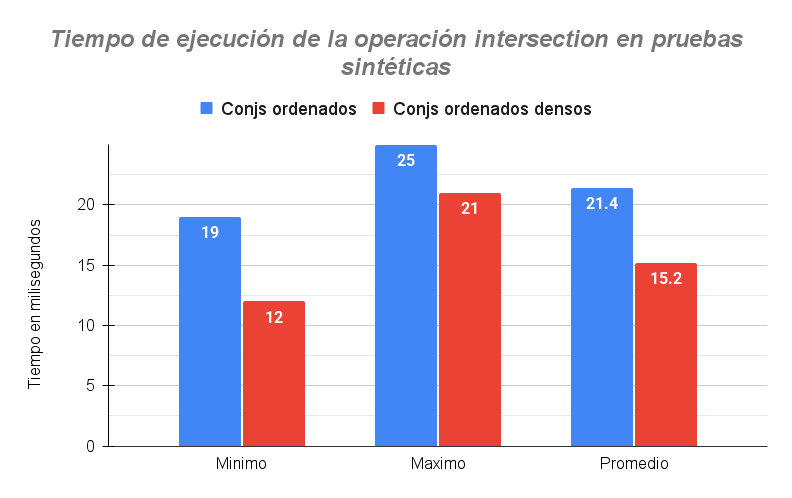
\includegraphics[width=0.8\linewidth]{figures/Rendimiento/sin/Tiempo de ejecución de la operación intersection en pruebas sintéticas.png}}
            \caption{Comparación entre conjuntos ordenados y conjuntos densos.}
          \end{subfigure}
          \vspace{0.8cm}
          \begin{subfigure}[b]{\linewidth}
            \centering
            \fbox{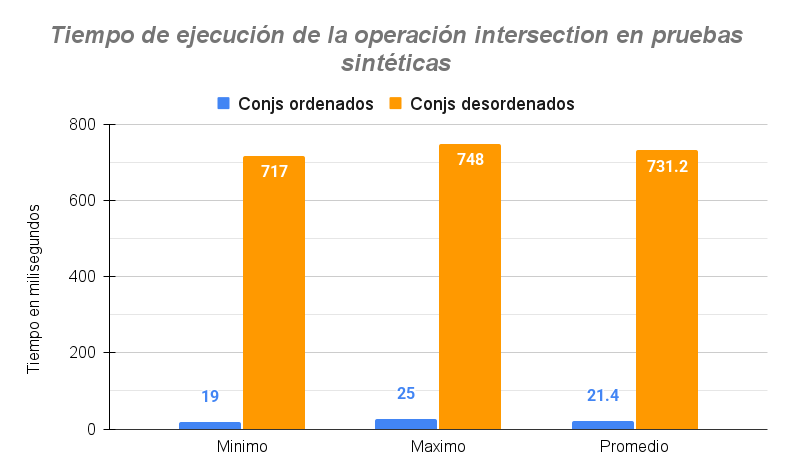
\includegraphics[width=0.8\linewidth]{figures/Rendimiento/sin/Tiempo de ejecución de la operación intersection en pruebas sintéticas (1).png}}
            \caption{Comparación entre conjuntos ordenados y conjuntos desordenados.}
          \end{subfigure}
          \caption{Comparación del tiempo de ejecución de la operación \texttt{intersection} entre las distintas implementaciones de conjuntos.}
          \label{fig:Ren-Int}
        \end{figure}

       \begin{table}[ht]
        \centering
        \fbox{%
        \begin{tabularx}{0.85\textwidth}{|c|>{\centering\arraybackslash}X|>{\centering\arraybackslash}X|}
        \hline
        \textbf{} & \multicolumn{2}{c|}{\parbox[c]{0.45\textwidth}{\centering \textbf{Tiempo de ejecución en milisegundos}}} \\
        \hline
        \textbf{Cantidad de multi-intervalos} & \textbf{Conjuntos ordenados} & \textbf{Conjuntos desordenados} \\
        \hline
        2000   & 8     & 41     \\
        \hline
        4000   & 18    & 134    \\
        \hline
        8000   & 28    & 476    \\
        \hline
        16000  & 36    & 1853   \\
        \hline
        32000  & 62    & 7553   \\
        \hline
        64000  & 137   & 32203  \\
        \hline
        \end{tabularx}}
        \caption{Cuadro de escalado del tiempo de ejecución de la operación \texttt{intersection}}
        \label{tab:Ren-Int-scal}
        \end{table}


        \begin{figure}[htbp]
          \centering
          \fbox{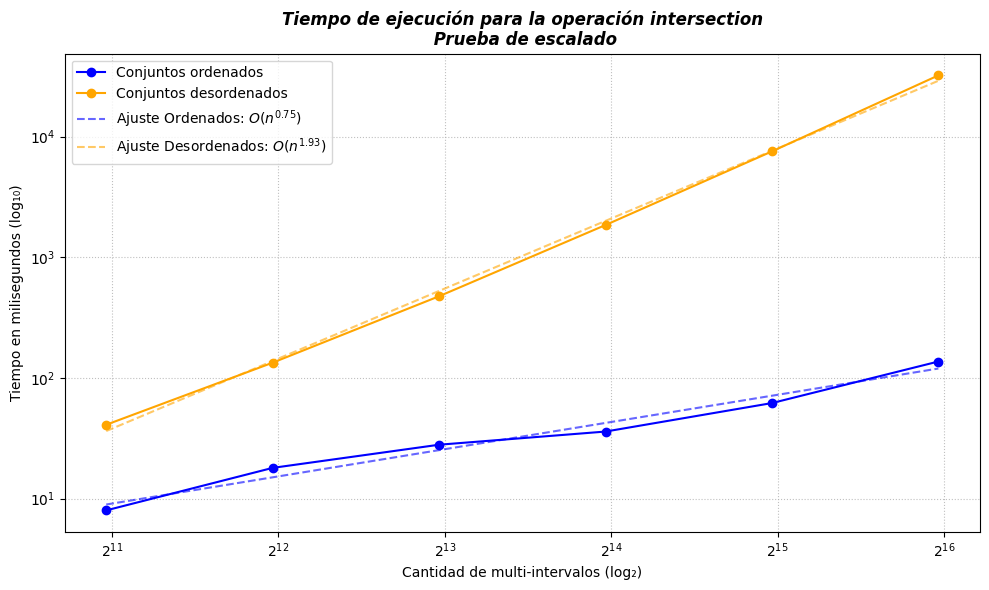
\includegraphics[width=0.9\linewidth]{figures/Rendimiento/sin/scal1.png}}
          \caption{Gráfica del escalado en el tiempo de ejecución de la operación \texttt{intersection}.}
          \label{fig:Ren-Int-scal2}
        \end{figure}

        \item \texttt{complement:} 
        Esta operación cuenta con una implementación específica para conjuntos ordenados. Tal como se muestra en la Figura~\ref{fig:Ren-Comp}, su rendimiento se sitúa entre el de las otras dos variantes, con una reducción relativa del tiempo de ejecución del \textbf{28{.}75\%} respecto a la versión desordenada.

        \begin{figure}[htbp]
          \centering
          \fbox{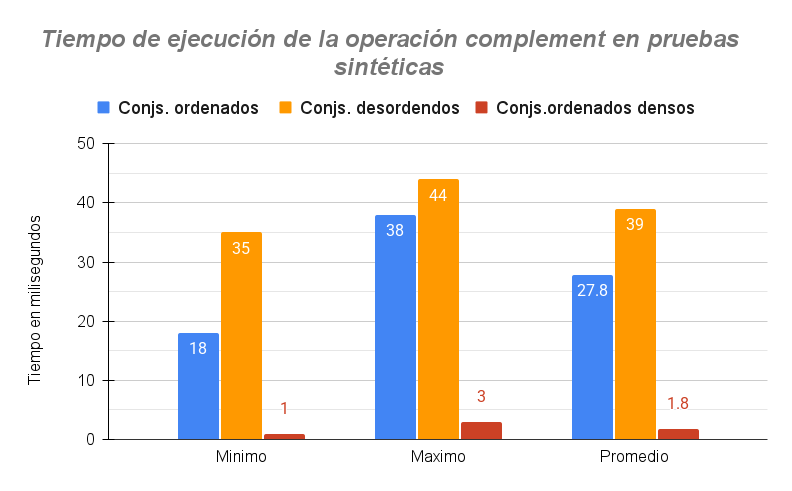
\includegraphics[width=0.8\linewidth]{figures/Rendimiento/sin/Tiempo de ejecución de la operación complement en pruebas sintéticas.png}}
          \caption{Comparación del tiempo de ejecución de la operación \texttt{complement}.}
          \label{fig:Ren-Comp}
        \end{figure}

        \item \texttt{disjointCup:} 
        En el caso de la operación \texttt{disjointCup} se preveía un rendimiento inferior en la implementación para conjuntos ordenados debido al costo del ordenamiento. Pero, gracias al \textbf{criterio de ordenamiento} aplicado, se logró un rendimiento similar para conjuntos ordenados que para conjuntos ordenados densos. Teniendo un aumento relativo del tiempo de ejecución del \textbf{40{.}82\%} respecto a la versión desordenada (ver Figura~\ref{fig:Ren-dis}). Eso se debe que la implementación desordenado no realiza procedimiento adicional mas allá de la inserción de los elementos.

        \begin{figure}[htbp]
          \centering
          \fbox{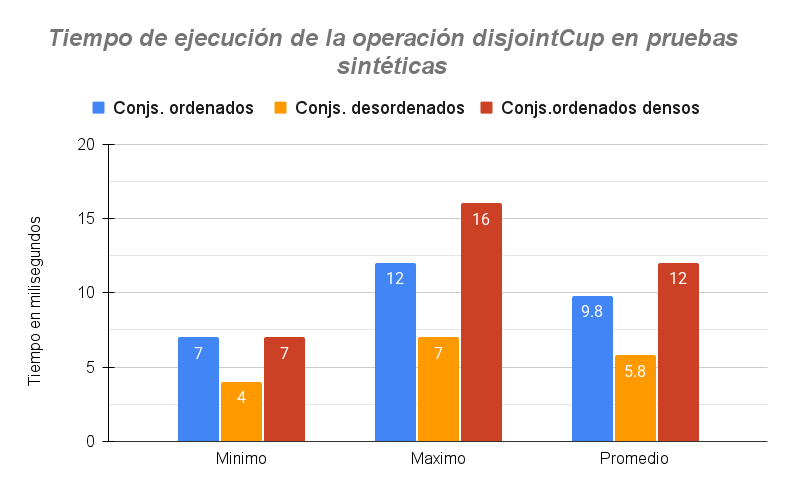
\includegraphics[width=0.8\linewidth]{figures/Rendimiento/sin/Tiempo de ejecución de la operación disjointCup en pruebas sintéticas (1).png}}
          \caption{Comparación del tiempo de ejecución de la operación \texttt{disjointCup}.}
          \label{fig:Ren-dis}
        \end{figure}

        \item \texttt{cup:} 
        Al estar implementada a partir de otras operaciones, la eficiencia de \texttt{cup} depende directamente de estas. La implementación sobre conjuntos ordenados muestra una mejora del \textbf{26{.}09\%} en el tiempo de ejecución respecto a la versión con conjuntos desordenados (ver Figura~\ref{fig:Ren-cup}).

        \begin{figure}[htbp]
          \centering
          \fbox{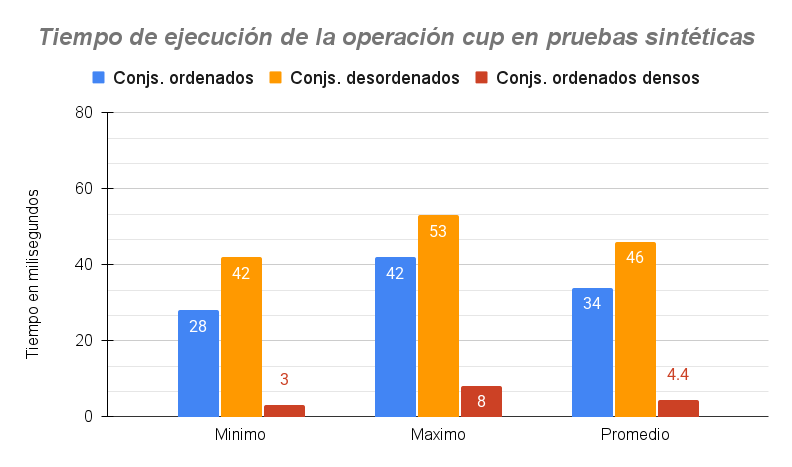
\includegraphics[width=0.8\linewidth]{figures/Rendimiento/sin/Tiempo de ejecución de la operación cup en pruebas sintéticas.png}}
          \caption{Comparación del tiempo de ejecución de la operación \texttt{cup}.}
          \label{fig:Ren-cup}
        \end{figure}

        \item \texttt{difference:} 
        Similar a \texttt{cup}, esta operación se basa en funciones auxiliares. La versión con conjuntos ordenados reduce el tiempo de ejecución en un \textbf{19{.}05\%} en comparación con la implementación desordenada (ver Figura~\ref{fig:Ren-dif}).

        \begin{figure}[htbp]
          \centering
          \fbox{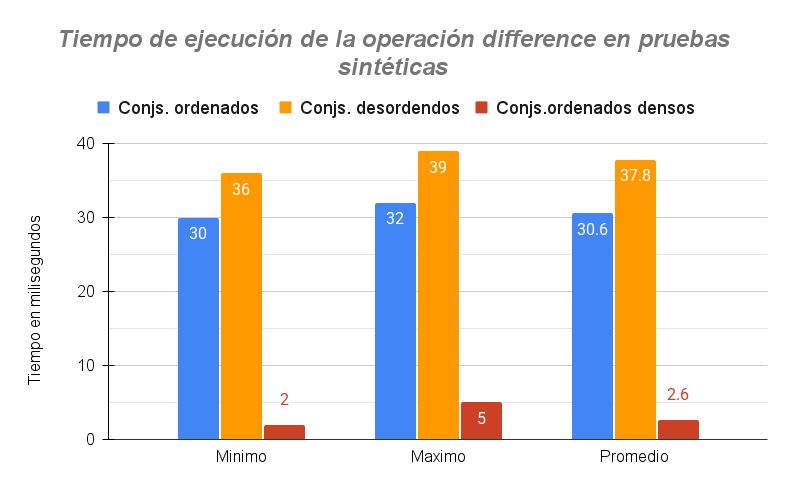
\includegraphics[width=0.8\linewidth]{figures/Rendimiento/sin/Tiempo de ejecución de la operación difference en pruebas sintéticas.png}}
          \caption{Comparación del tiempo de ejecución de la operación \texttt{difference}.}
          \label{fig:Ren-dif}
        \end{figure}
    \end{itemize}

    En promedio, las implementaciones para conjuntos ordenados alcanza una mejora palpable frente a la versión desordenada al trabajar con conjuntos unidimensionales densos, con excepción de la operación \texttt{intersection}, donde la mejora fue especialmente destacada y \texttt{disjointCup} donde la pérdida era esperable.

    A continuación, se analiza el rendimiento sobre conjuntos con multi-intervalos tridimensionales y con paso variable, para evaluar el comportamiento en un contexto más general.

    \item \textbf{\textit{Casos de prueba sintéticos tridimensionales y no densos:}}

    En este escenario, se utilizaron conjuntos de 1.000 multi-intervalos con tres dimensiones y con paso dos en la primera dimensión, comparando en esta ocasión la implementación ordenada frente a la desordenada.

    \begin{itemize}
        \item \texttt{intersection:} 
        Aunque la diferencia de rendimiento no es tan marcada como en el caso unidimensional, debido a la cantidad de elementos de los conjuntos, la versión ordenada logra una reducción relativa del \textbf{58{.}82\%} en el tiempo de ejecución (Figura~\ref{fig:Ren-int-3d}).

        \begin{figure}[htbp]
          \centering
          \fbox{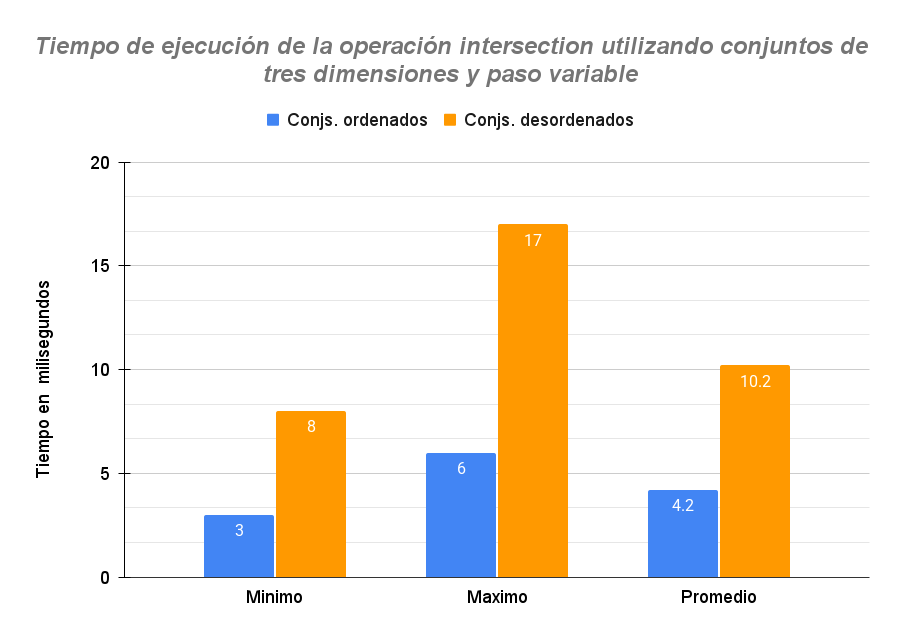
\includegraphics[width=0.8\linewidth]{figures/Rendimiento/sin/Tiempo de ejecución de la operación intersection utilizando conjuntos de tres dimensiones y paso variable.png}}
          \caption{Tiempo de ejecución de \texttt{intersection} con conjuntos tridimensionales con paso distinto de 1, comparando conjuntos ordenados y desordenados.}
          \label{fig:Ren-int-3d}
        \end{figure}

        \item \texttt{complement:} 
        En este caso, la optimizaciones permiten aprovechar las múltiples dimensiones disponibles para alcanzar una reducción relativa del \textbf{98{.}87\%}, lo que representa una mejora de aproximadamente \textbf{88{.}10 veces} (Figura~\ref{fig:Ren-comp-3d}).

         En cuanto al análisis de escalabilidad de esta operación, se observa que la implementación que utiliza conjuntos ordenados presenta un escalado aproximadamente lineal o sublineal, al aumentar la cantidad de multi-intervalos. En contraste, este comportamiento no se mantiene al utilizar la versión basada en conjuntos desordenados, como se muestra en la Figura~\ref{fig:Ren-comp-3d-scal2}, cuyos datos previenen del Cuadro~\ref{tab:Ren-comp-3d-scal2}.
        
        \begin{figure}[htbp]
          \centering
          \fbox{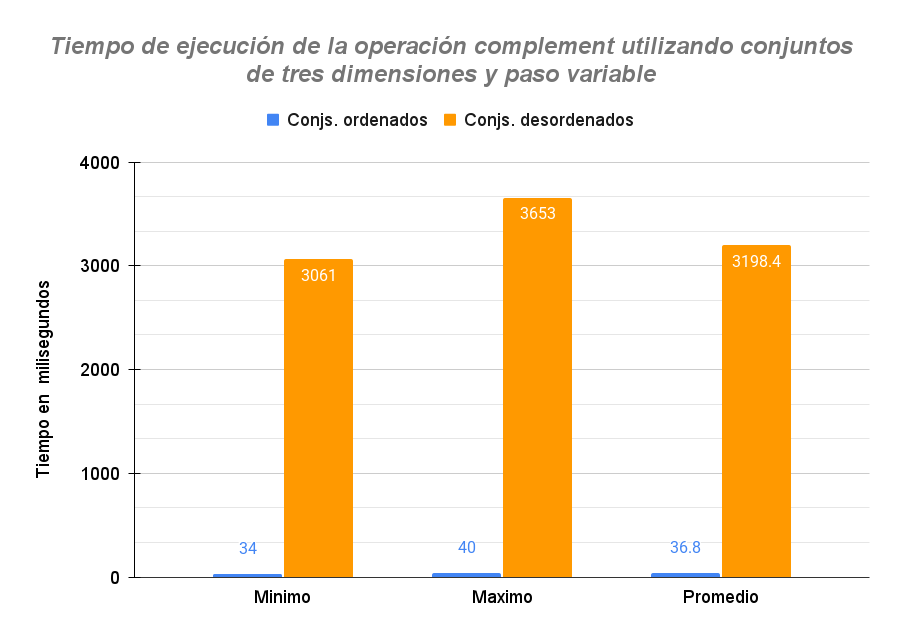
\includegraphics[width=0.8\linewidth]{figures/Rendimiento/sin/Tiempo de ejecución de la operación complement utilizando conjuntos de tres dimensiones y paso variable.png}}
          \caption{Tiempo de ejecución de \texttt{complement} con conjuntos tridimensionales con paso distinto de 1, comparando conjuntos ordenados y desordenados.}
          \label{fig:Ren-comp-3d}
        \end{figure}

        \begin{table}[ht]
        \centering
        \fbox{%
    \begin{tabularx}{0.85\textwidth}{|c|>{\centering\arraybackslash}X|>{\centering\arraybackslash}X|}
    \hline
\textbf{} & \multicolumn{2}{c|}{\textbf{Tiempo de ejecución en milisegundos}} \\
\hline
        \textbf{Cantidad de multi-intervalos} & \textbf{Conjuntos ordenados} & \textbf{Conjuntos desordenados} \\
        \hline
        250    & 13     & 249      \\
        \hline
        500    & 23     & 813      \\
        \hline
        1000   & 26     & 3165     \\
        \hline
        2000   & 58     & 12392    \\
        \hline
        4000   & 107    & 50184    \\
        \hline
        8000   & 192    & 200823   \\
        \hline
        \end{tabularx}}
        \caption{Cuadro de escalado del tiempo de ejecución de la operación \texttt{complement}}
        \label{tab:Ren-comp-3d-scal2}
        \end{table}

      
        \begin{figure}[htbp]
          \centering
          \fbox{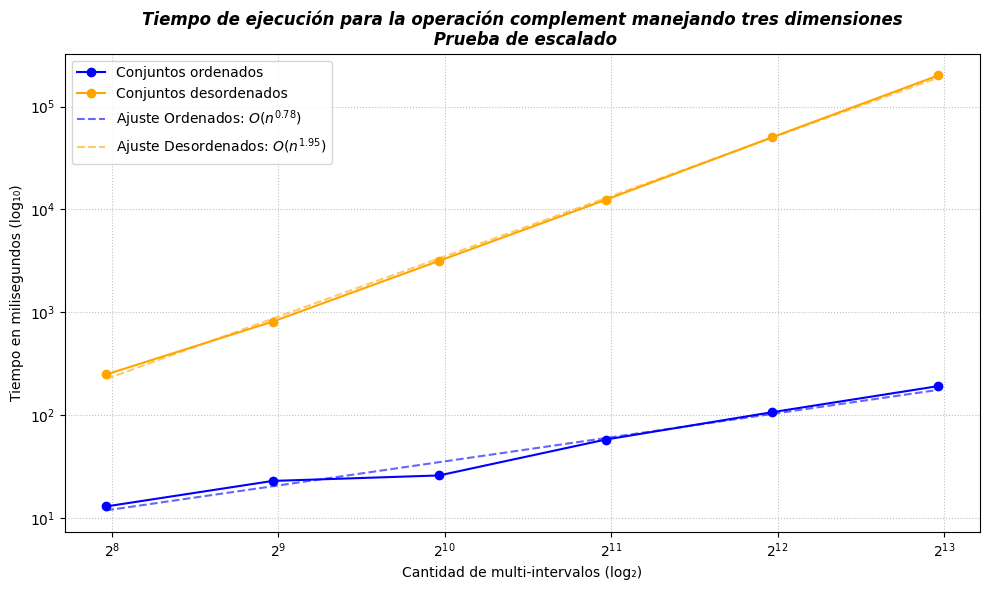
\includegraphics[width=1\linewidth]{figures/Rendimiento/sin/scal2.png}}
          \caption{Análisis del escalado en el tiempo de ejecución de la operación \texttt{complement}.}
          \label{fig:Ren-comp-3d-scal2}
        \end{figure}

        \item \texttt{cup:} 
        Dependiente de \texttt{complement}, esta operación se beneficia de sus optimizaciones, logrando una mejora del \textbf{97{.}93\%} o \textbf{48{.}41 veces} más rápido que la versión desordenada (Figura~\ref{fig:Ren-cup-3d}).


        \begin{figure}[htbp]
          \centering
          \fbox{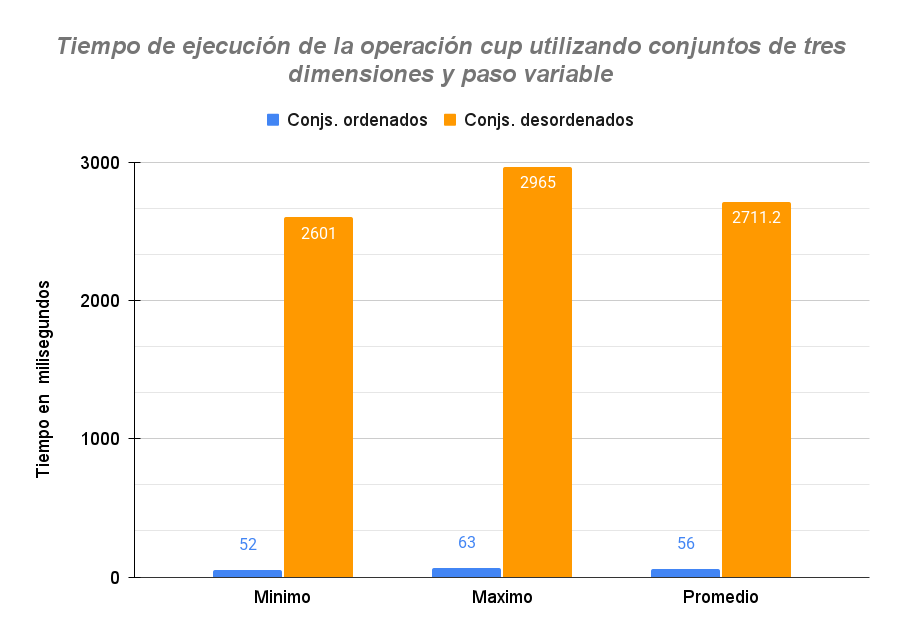
\includegraphics[width=0.9\linewidth]{figures/Rendimiento/sin/Tiempo de ejecución de la operación cup utilizando conjuntos de tres dimensiones y paso variable.png}}
          \caption{Tiempo de ejecución de \texttt{cup} con conjuntos tridimensionales con paso distinto de 1, comparando conjuntos ordenados y desordenados.}
          \label{fig:Ren-cup-3d}
        \end{figure}

        \item \texttt{difference:} 
        También construida sobre otras operaciones, \texttt{difference} logra una mejora del \textbf{98\%}, equivalente a una ejecución \textbf{50{.}15 veces} más rápida que la versión desordenada (Figura~\ref{fig:Ren-dif-3d}).

        \begin{figure}[htbp]
          \centering
          \fbox{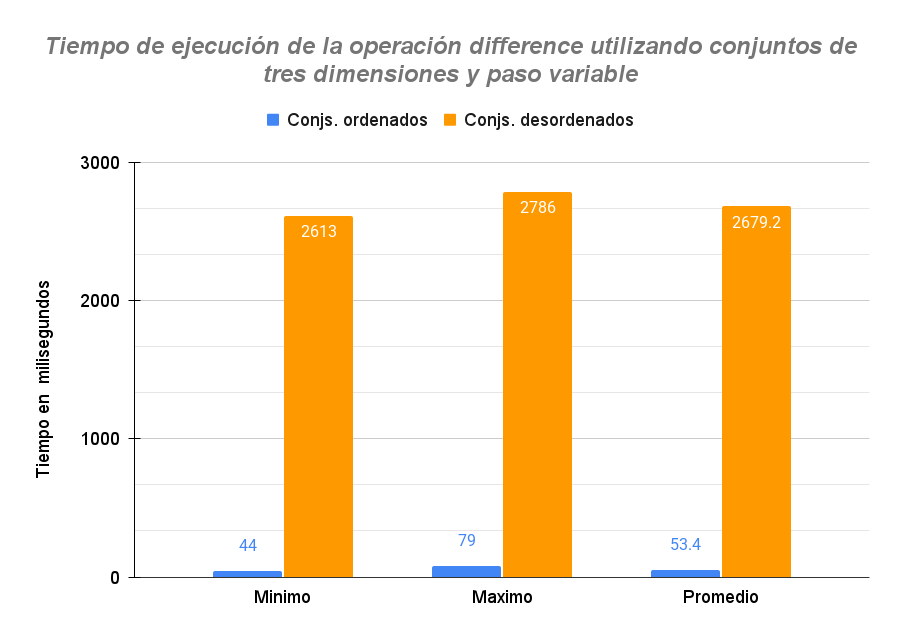
\includegraphics[width=0.8\linewidth]{figures/Rendimiento/sin/Tiempo de ejecución de la operación difference utilizando conjuntos de tres dimensiones y paso variable.png}}
          \caption{Tiempo de ejecución de \texttt{difference} con conjuntos tridimensionales con paso distinto de 1, comparando conjuntos ordenados y desordenados.}
          \label{fig:Ren-dif-3d}
        \end{figure}

         \item \texttt{disjointCup:} 
        Nuevamente se puede ver como se tiene un empeoramiento en el rendimiento de la operación \texttt{disjointCup} para conjuntos ordenandos con respecto a la misma para conjuntos desordenados. 
         Se obtiene entonces un aumento relativo del tiempo de ejecución del \textbf{75{.}61\%} respecto a la versión desordenada (Ver Figura~\ref{fig:Ren-dis-3d}). Esta prueba es la única dentro de este apartado en la cual se usaron 5000 multi-intervalos por conjunto.

        \begin{figure}[htbp]
          \centering
          \fbox{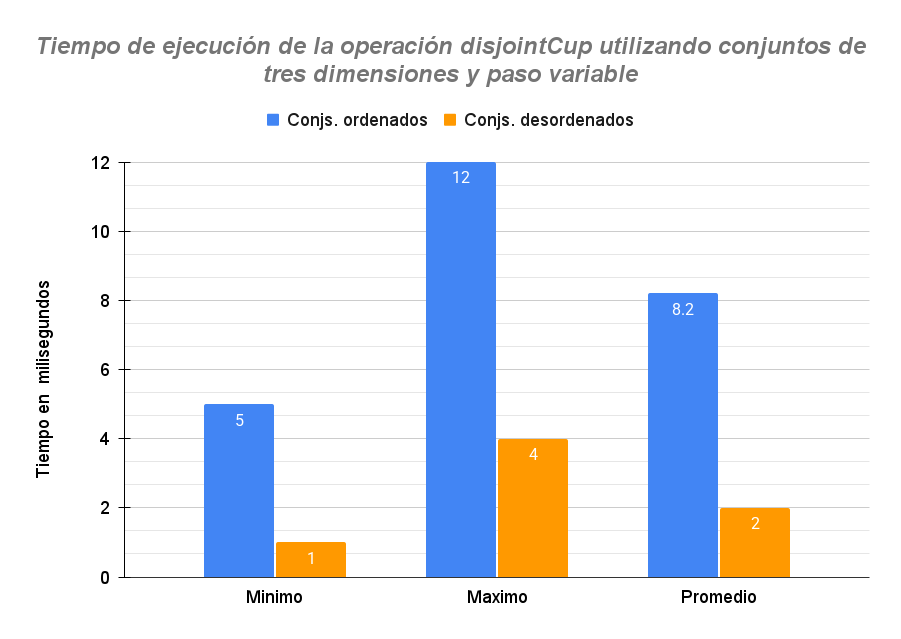
\includegraphics[width=0.8\linewidth]{figures/Rendimiento/sin/Tiempo de ejecución de la operación disjointCup utilizando conjuntos de tres dimensiones y paso variable.png}}
          \caption{Tiempo de ejecución de \texttt{disjointCup} con conjuntos tridimensionales con paso distinto de 1, comparando conjuntos ordenados y desordenados.}
          \label{fig:Ren-dis-3d}
        \end{figure}
    \end{itemize}
\end{itemize}


\section{Casos de prueba sintéticos para \textit{piecewise maps} ordenados}

Al igual que en la sección anterior, se diseñó un conjunto extenso de casos de prueba 
sintéticos para las operaciones de los \textit{piecewise maps}, con el propósito de 
evaluar el rendimiento de las dos implementaciones disponibles.  

De manera análoga, se presentan a continuación los resultados obtenidos, junto con una 
comparación detallada entre las variantes de \textit{piecewise maps} ordenados y 
desordenados. Los valores representados en las gráficas corresponden al 
\textbf{mínimo}, \textbf{máximo} y \textbf{promedio} de los tiempos de ejecución 
registrados tras múltiples repeticiones de cada caso de prueba sintético, tal como se 
procedió en la sección anterior. Además, al igual que entonces, todos los porcentajes 
y comparaciones mostrados se calcularon sobre los valores \textbf{promedio}, 
\textit{excepto en las pruebas de escalabilidad}, donde solo se dio una ejecución de los casos por las cantidad de mapas.

Cabe señalar que, en esta ocasión, no se considerarán casos de prueba en una única 
dimensión, dado que, tal como se observó en el análisis de los conjuntos, las 
optimizaciones no aportan mejoras significativas en dicho contexto. Por lo tanto, 
se trabajará exclusivamente con tres dimensiones. Adicionalmente, a diferencia que en el caso de conjuntos, cada caso de prueba sintéticos maneja argumentos muy distintos entre si. Por lo que si se desea ver estos en profundidad se debe chequear el archivo \textit{pwmap\_perf.cpp} en la carpeta \textit{tests/performance} dentro del repositorio. 

\begin{itemize}
   \item \texttt{combine:} 
La primera operación que se analizará es \texttt{combine}, la cual, por su propia 
naturaleza, se presenta como una candidata a no resultar más eficiente en los 
\textit{piecewise maps} ordenados. En la Figura~\ref{fig:Ren-com-3d} se observa una reducción del rendimiento de la versión ordenada en comparación con la desordenada. 
En este caso, el tiempo de ejecución muestra un incremento relativo del 
\textbf{42{,}89\%} con respecto a la implementación desordenada.

   \begin{figure}[htbp]
          \centering
          \fbox{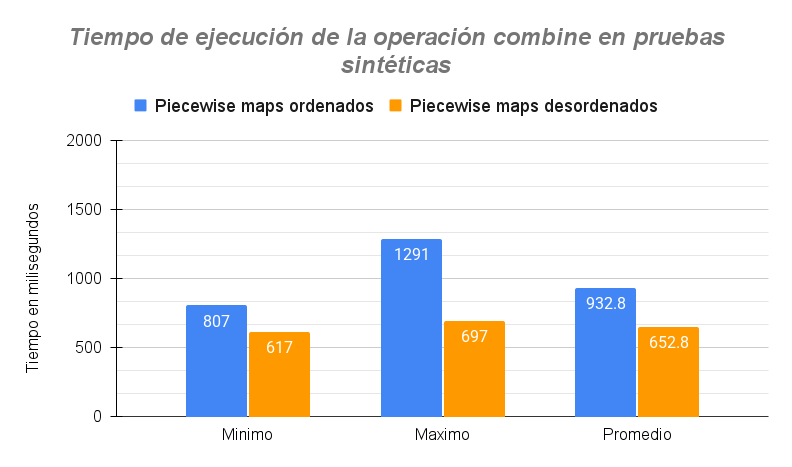
\includegraphics[width=0.8\linewidth]{figures/Rendimiento/pwm/Tiempo de ejecución de la operación combine en pruebas sintéticas.png}}
          \caption{Tiempo de ejecución de \texttt{combine} utilizando tres dimensiones, comparando \textit{piecewise maps} ordenados y desordenados.}
          \label{fig:Ren-com-3d}
        \end{figure}


       \item \texttt{concatenation:} 
        Esta es otra de las operaciones en las que, debido a su propia naturaleza, 
        el orden resulta desfavorable. En la Figura~\ref{fig:Ren-concat-3d} 
        se observa que la versión para los \textit{piecewise maps} ordenados 
        presenta un incremento relativo en el tiempo de ejecución del 
        \textbf{16{,}22\%} en comparación con la versión desordenada.


   \begin{figure}[htbp]
          \centering
          \fbox{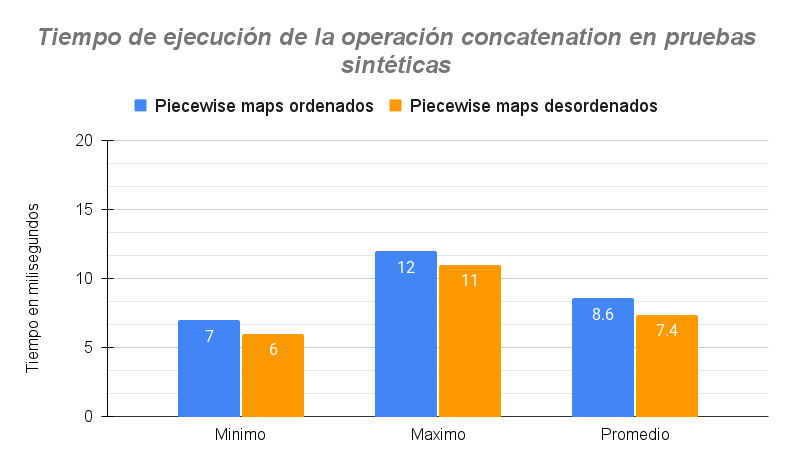
\includegraphics[width=0.8\linewidth]{figures/Rendimiento/pwm/Tiempo de ejecución de la operación concatenation en pruebas sintéticas.png}}
          \caption{Tiempo de ejecución de \texttt{concatenation} utilizando tres dimensiones, comparando \textit{piecewise maps} ordenados y desordenados.}
          \label{fig:Ren-compo-3d}
        \end{figure}

           \item \texttt{restrict:} 
            A continuación se analiza la operación \texttt{restrict}, la cual en este caso 
            sí presenta una mejora. En la Figura~\ref{fig:Ren-rest-3d} se observa que, 
            aunque la ganancia no es muy significativa, la versión ordenada logra una 
            disminución relativa del tiempo de ejecución del \textbf{13{,}82\%} en comparación 
            con la versión desordenada.



   \begin{figure}[htbp]
          \centering
          \fbox{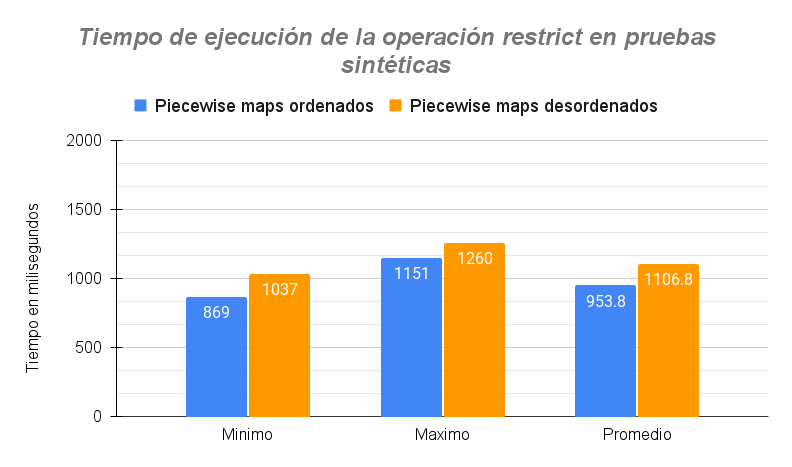
\includegraphics[width=0.8\linewidth]{figures/Rendimiento/pwm/Tiempo de ejecución de la operación restrict en pruebas sintéticas.png}}
          \caption{Tiempo de ejecución de \texttt{restrict} utilizando tres dimensiones, comparando \textit{piecewise maps} ordenados y desordenados.}
          \label{fig:Ren-rest-3d}
        \end{figure}

    En el Cuadro~\ref{tab:restrict-esc} y en la Figura~\ref{fig:restrict-esc} 
    se evidencia que, incluso con las optimizaciones introducidas en la versión ordenada, ambas implementaciones presentan un escalado similar. No obstante, puede apreciarse que la versión ordenada logra un desempeño levemente superior en términos de escalabilidad.



    \begin{table}[ht]
    \centering
    \fbox{%
    \begin{tabularx}{0.75\textwidth}{|c|>{\centering\arraybackslash}X|>{\centering\arraybackslash}X|}
    \hline
\textbf{} & \multicolumn{2}{c|}{\textbf{Tiempo de ejecución en milisegundos}} \\
\hline
    \textbf{Cantidad de mapas} & \textbf{Piecewise maps ordenados} & \textbf{Piecewise maps desordenados} \\
    \hline
    16   & 3    & 3    \\
    \hline
    32   & 7    & 12   \\
    \hline
    64   & 25   & 27   \\
    \hline
    128  & 94   & 106  \\
    \hline
    256  & 370  & 424  \\
    \hline
    512  & 1469 & 1665 \\
    \hline
    1024 & 5846 & 6725 \\
    \hline
    \end{tabularx}}
    \caption{Cuadro de escalado del tiempo de ejecución de la operación \texttt{restrict}}
    \label{tab:restrict-esc}
    \end{table}

    \begin{figure}[htbp]
          \centering
          \fbox{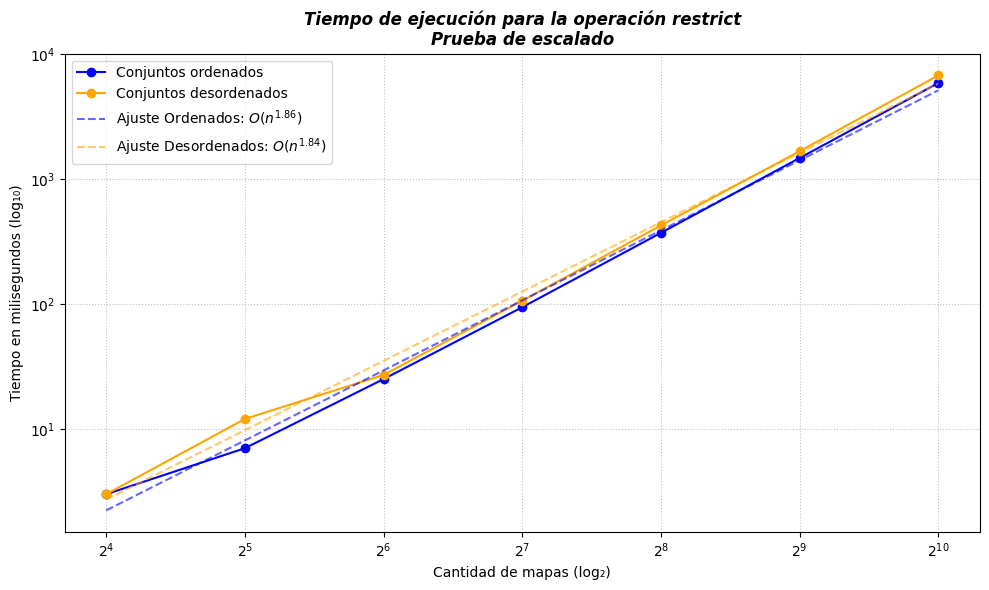
\includegraphics[width=1\linewidth]{figures/Rendimiento/pwm/scal4.png}}
          \caption{Análisis del escalado en el tiempo de ejecución de la operación \texttt{restrict}.}
          \label{fig:restrict-esc}
    \end{figure}


        \item \texttt{composition:} 
        El caso de la operación \texttt{composition} resulta particularmente interesante, 
        ya que su implementación, en términos generales, incluye un doble ciclo \textit{for}. En la 
        Figura~\ref{fig:Ren-compo-3d} se aprecia la marcada diferencia en el rendimiento 
        entre ambas versiones. En este caso, la versión ordenada logra una reducción 
        relativa del tiempo de ejecución del \textbf{92{,}63\%} en comparación con la 
        versión desordenada.



   \begin{figure}[htbp]
          \centering
          \fbox{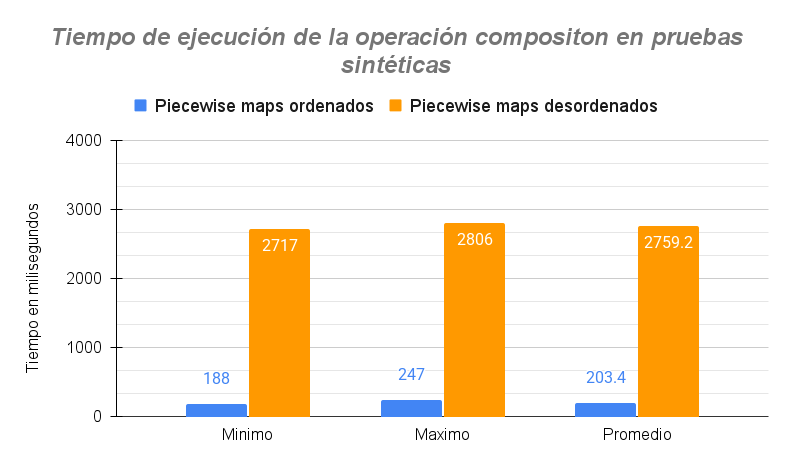
\includegraphics[width=0.8\linewidth]{figures/Rendimiento/pwm/Tiempo de ejecución de la operación compositon en pruebas sintéticas.png}}
          \caption{Tiempo de ejecución de \texttt{composition} utilizando tres dimensiones, comparando \textit{piecewise maps} ordenados y desordenados.}
          \label{fig:Ren-concat-3d}
        \end{figure}

    En el Cuadro~\ref{tab:composition-esc} y en la Figura~\ref{fig:composition-esc} 
    se observa que la operación implementada para los \textit{piecewise maps} ordenados presenta un mejor escalado en comparación con la implementación desordenada. 
    Sin embargo, aún está un poco lejos de alcanzar un comportamiento verdaderamente lineal.



    \begin{table}[ht]
    \centering
    \fbox{%
    \begin{tabularx}{0.75\textwidth}{|c|>{\centering\arraybackslash}X|>{\centering\arraybackslash}X|}
    \hline
\textbf{} & \multicolumn{2}{c|}{\textbf{Tiempo de ejecución en milisegundos}} \\
\hline
    \textbf{Cantidad de mapas} & \textbf{Piecewise maps ordenados} & \textbf{Piecewise maps desordenados} \\
    \hline
    16   & 40    & 98     \\
    \hline
    32   & 63    & 315    \\
    \hline
    64   & 123   & 1164   \\
    \hline
    128  & 244   & 4423   \\
    \hline
    256  & 594   & 17240  \\
    \hline
    512  & 2776  & 68963  \\
    \hline
    1024 & 7822  & 272032 \\
    \hline
    \end{tabularx}}
    \caption{Cuadro de escalado del tiempo de ejecución de la operación \texttt{composition}}
    \label{tab:composition-esc}
    \end{table}

    \begin{figure}[htbp]
          \centering
          \fbox{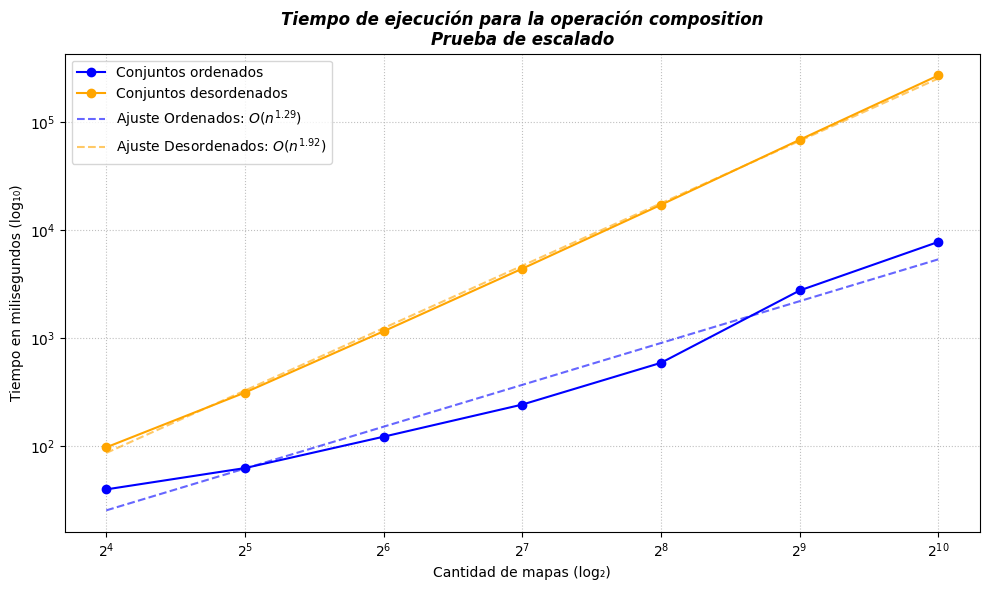
\includegraphics[width=1\linewidth]{figures/Rendimiento/pwm/scal3.png}}
          \caption{Análisis del escalado en el tiempo de ejecución de la operación \texttt{composition}.}
          \label{fig:composition-esc}
    \end{figure}

            \item \texttt{offsetDom:} 
        En este caso nuevamente se evidencia una mejora significativa al emplear el orden. 
        En la Figura~\ref{fig:Ren-off-3d} se observa que la versión ordenada logra una 
        reducción relativa del tiempo de ejecución del \textbf{46{,}31\%} en comparación 
        con la versión desordenada.


   \begin{figure}[htbp]
          \centering
          \fbox{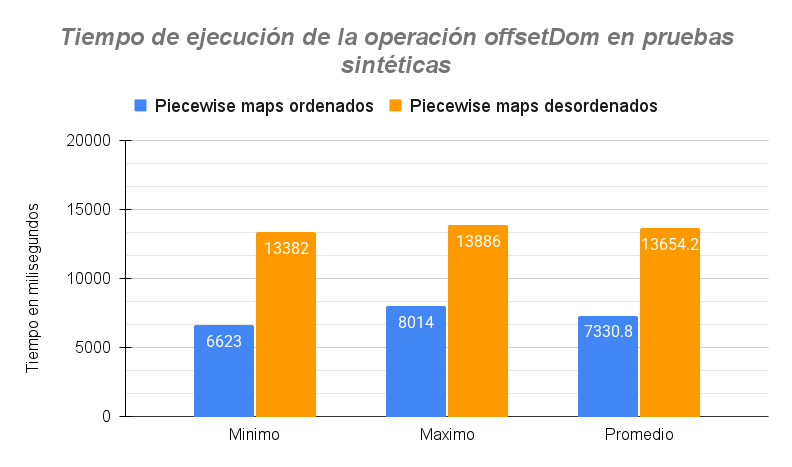
\includegraphics[width=0.8\linewidth]{figures/Rendimiento/pwm/Tiempo de ejecución de la operación offsetDom en pruebas sintéticas.png}}
          \caption{Tiempo de ejecución de \texttt{offsetDom} utilizando tres dimensiones, comparando \textit{piecewise maps} ordenados y desordenados.}
          \label{fig:Ren-off-3d}
        \end{figure}

    \item \texttt{firstInv:} 
    El caso de la operación \texttt{firstInv} resulta particularmente peculiar. 
    En la Figura~\ref{fig:Ren-firstInv-3d} se observa que ambas versiones de la 
    operación presentan un rendimiento prácticamente equivalente, con una reducción 
    relativa del tiempo de ejecución de apenas \textbf{2{,}73\%} en la versión 
    ordenada respecto de la desordenada.

   \begin{figure}[htbp]
          \centering
          \fbox{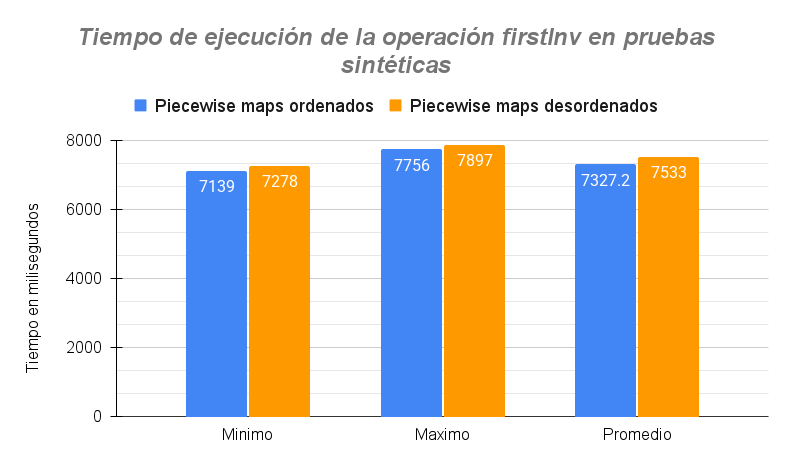
\includegraphics[width=0.8\linewidth]{figures/Rendimiento/pwm/Tiempo de ejecución de la operación firstInv en pruebas sintéticas.png}}
          \caption{Tiempo de ejecución de \texttt{firstInv} utilizando tres dimensiones, comparando \textit{piecewise maps} ordenados y desordenados.}
          \label{fig:Ren-firstInv-3d}
        \end{figure}

    \item \texttt{+:} 
    Con la operación de suma se da inicio a aquellas que se benefician del 
    uso de la función \texttt{processMapsOrd}. En particular, en la 
    Figura~\ref{fig:Ren-suma-3d} se observa una reducción relativa del tiempo de 
    ejecución del \textbf{95{,}89\,\%} en comparación con la implementación de los 
    \textit{piecewise maps} desordenados, siendo la versión ordenada aproximadamente 
    \textbf{24,35} veces más rápida.

    \begin{figure}[htbp]
          \centering
          \fbox{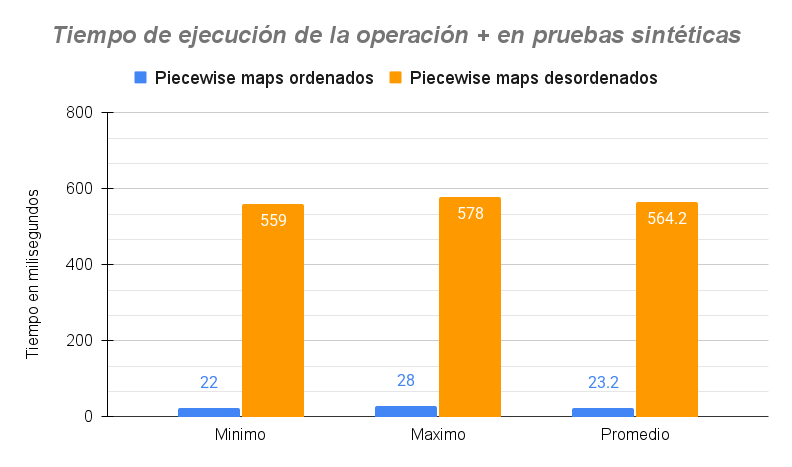
\includegraphics[width=0.8\linewidth]{figures/Rendimiento/pwm/Tiempo de ejecución de la operación + en pruebas sintéticas.png}}
          \caption{Tiempo de ejecución de \texttt{+} utilizando tres dimensiones, comparando \textit{piecewise maps} ordenados y desordenados.}
          \label{fig:Ren-suma-3d}
    \end{figure}

    En el Cuadro~\ref{tab:suma-esc} y en la Figura~\ref{fig:suma-esc} 
    se observa cómo la operación de suma varía significativamente en su 
    escalado entre las distintas versiones. En este caso, la versión implementada 
    para los \textit{piecewise maps} ordenados presenta un escalado mucho más 
    eficiente que la versión desordenada, mostrando un escaldo lineal.


    \begin{table}[ht]
    \centering
    \fbox{%
    \begin{tabularx}{0.75\textwidth}{|c|>{\centering\arraybackslash}X|>{\centering\arraybackslash}X|}
    \hline
\textbf{} & \multicolumn{2}{c|}{\textbf{Tiempo de ejecución en milisegundos}} \\
\hline
    \textbf{Cantidad de mapas} & \textbf{Piecewise maps ordenados} & \textbf{Piecewise maps desordenados} \\
    \hline
    16    & 4     & 11     \\
    \hline
    32    & 7     & 23     \\
    \hline
    64    & 7     & 68     \\
    \hline
    128   & 14    & 240    \\
    \hline
    256   & 28    & 939    \\
    \hline
    512   & 58    & 3771   \\
    \hline
    1024  & 131   & 15424  \\
    \hline
    \end{tabularx}}
    \caption{Cuadro de escalado del tiempo de ejecución de la operación \texttt{+}}
    \label{tab:suma-esc}
    \end{table}

    \begin{figure}[htbp]
          \centering
          \fbox{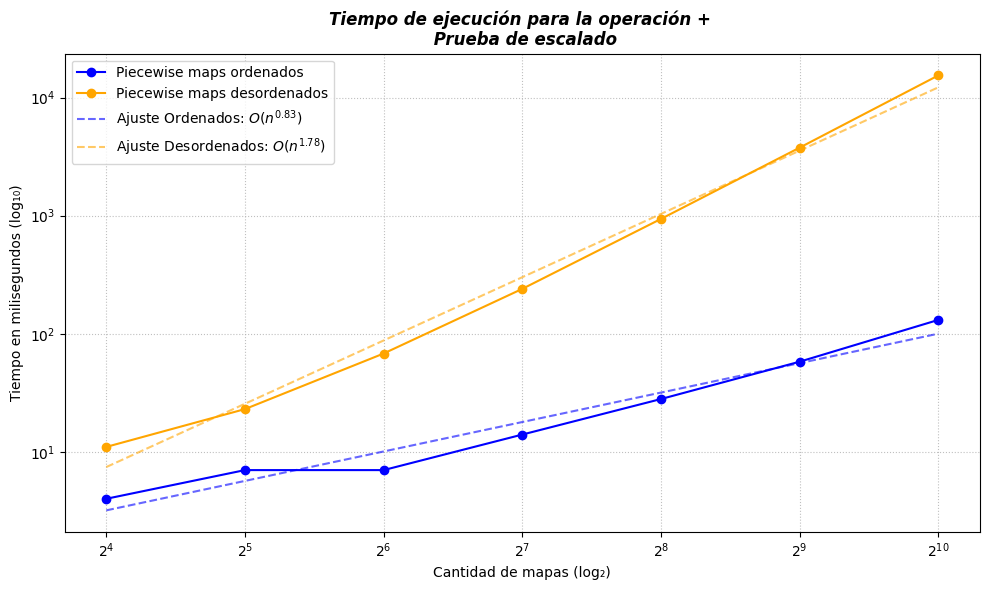
\includegraphics[width=1\linewidth]{figures/Rendimiento/pwm/scal1.png}}
          \caption{Análisis del escalado en el tiempo de ejecución de la operación \texttt{+}.}
          \label{fig:suma-esc}
    \end{figure}



    \item \texttt{-:} 
    El caso de la operación de \texttt{resta} no resulta tan desproporcionado como el 
    de la \texttt{suma}. En la Figura~\ref{fig:Ren-resta-3d} se observa que la versión 
    ordenada de los \textit{piecewise maps} logra una reducción relativa del tiempo de 
    ejecución del \textbf{80{,}15\,\%} con respecto a la implementación desordenada. Siendo \textbf{5} veces mas rápida.


   \begin{figure}[htbp]
          \centering
          \fbox{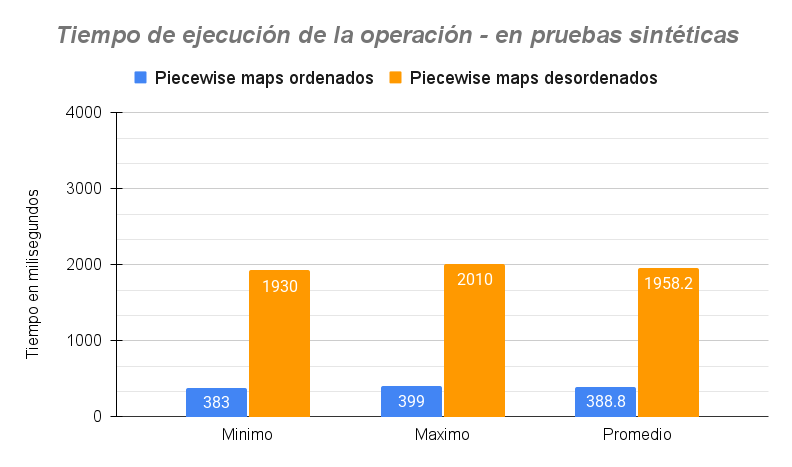
\includegraphics[width=0.8\linewidth]{figures/Rendimiento/pwm/Tiempo de ejecución de la operación - en pruebas sintéticas.png}}
          \caption{Tiempo de ejecución de \texttt{-} utilizando tres dimensiones, comparando \textit{piecewise maps} ordenados y desordenados.}
          \label{fig:Ren-resta-3d}
        \end{figure}
    \item \texttt{equalImage:} 
        Esta operación, al igual que la suma, se ve completamente optimizada gracias 
        al uso de la operación \texttt{processMapsOrd}. En la Figura~\ref{fig:Ren-equal-3d} 
        se aprecia una reducción relativa del tiempo de ejecución del \textbf{98{,}70\,\%} 
        con respecto a la versión desordenada, siendo la versión ordenada unas 
        \textbf{76.82} veces más rápida.



   \begin{figure}[htbp]
          \centering
          \fbox{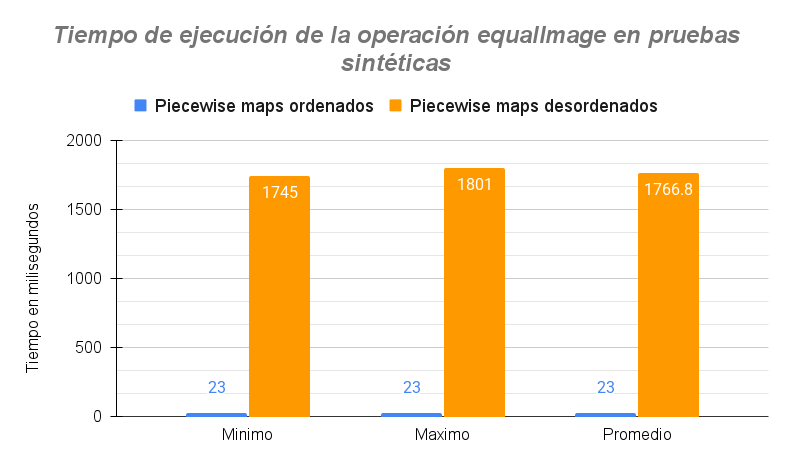
\includegraphics[width=0.8\linewidth]{figures/Rendimiento/pwm/Tiempo de ejecución de la operación equalImage en pruebas sintéticas.png}}
          \caption{Tiempo de ejecución de \texttt{equalImage} utilizando tres dimensiones, comparando \textit{piecewise maps} ordenados y desordenados.}
          \label{fig:Ren-equal-3d}
        \end{figure}

    \item \texttt{minAdjMap:} 
Se analiza finalmente la última operación, la cual nuevamente demuestra cómo el 
orden contribuye a mejorar el rendimiento. En la Figura~\ref{fig:Ren-min-3d} 
se evidencia una reducción relativa del tiempo de ejecución del 
\textbf{74{,}63\,\%} en comparación con la versión desordenada.




   \begin{figure}[htbp]
          \centering
          \fbox{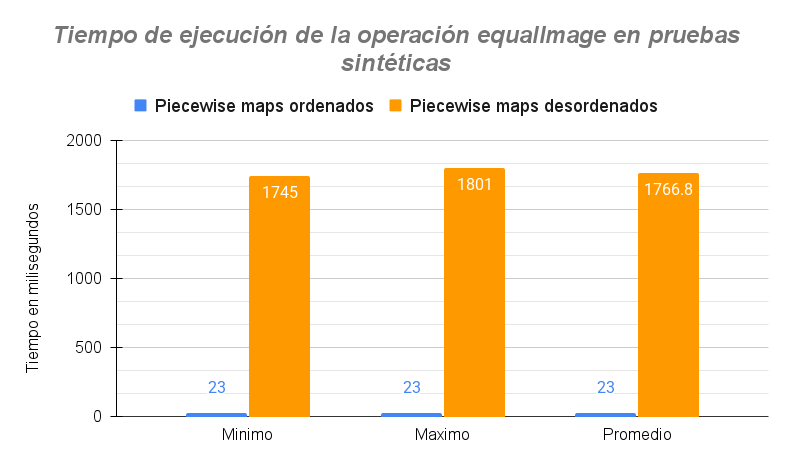
\includegraphics[width=0.8\linewidth]{figures/Rendimiento/pwm/Tiempo de ejecución de la operación equalImage en pruebas sintéticas.png}}
          \caption{Tiempo de ejecución de \texttt{minAdjMap} utilizando tres dimensiones, comparando \textit{piecewise maps} ordenados y desordenados.}
          \label{fig:Ren-min-3d}
        \end{figure}


    En el Cuadro~\ref{tab:min-esc} y en la Figura~\ref{fig:min-esc} 
    se observa que ambas versiones presentan un escalado similar, aunque la 
    versión que utiliza el orden muestra un comportamiento un poco más eficiente.



    \begin{table}[ht]
    \centering
    \fbox{%
    \begin{tabularx}{0.75\textwidth}{|c|>{\centering\arraybackslash}X|>{\centering\arraybackslash}X|}
    \hline
\textbf{} & \multicolumn{2}{c|}{\textbf{Tiempo de ejecución en milisegundos}} \\
\hline
    \textbf{Cantidad de mapas} & \textbf{Piecewise maps ordenados} & \textbf{Piecewise maps desordenados} \\
    \hline
    16    & 1      & 2      \\
    \hline
    32    & 7      & 15     \\
    \hline
    64    & 15     & 33     \\
    \hline
    128   & 37     & 98     \\
    \hline
    256   & 104    & 347    \\
    \hline
    512   & 375    & 1436   \\
    \hline
    1024  & 1473   & 5544   \\
    \hline
    \end{tabularx}}
    \caption{Cuadro de escalado del tiempo de ejecución de la operación \texttt{minAdjMap}}
    \label{tab:min-esc}
    \end{table}
    


    \begin{figure}[htbp]
          \centering
          \fbox{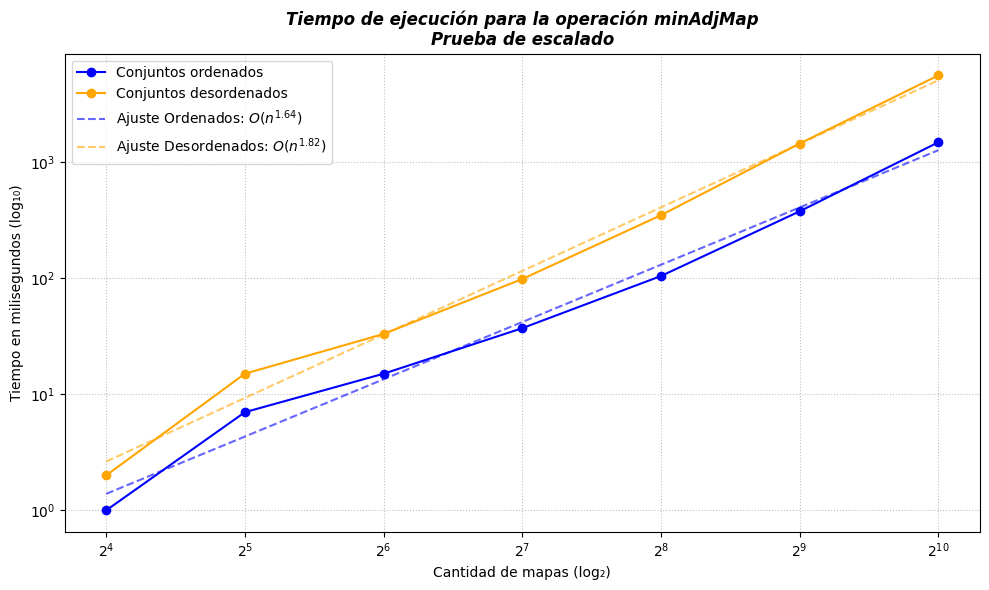
\includegraphics[width=1\linewidth]{figures/Rendimiento/pwm/scal2.png}}
          \caption{Análisis del escalado en el tiempo de ejecución de la operación \texttt{minAdjMap}.}
          \label{fig:min-esc}
    \end{figure}
\end{itemize}


\section{Casos de prueba}

En la sección anterior se trabajó con casos de prueba sintéticos para conjuntos, diseñados específicamente para verificar el rendimiento de las distintas operaciones sobre conjuntos en las diferentes implementaciones. Sin embargo, también resulta fundamental analizar cómo se desempeñan las implementaciones bajo condiciones más realistas. Dado que los conjuntos y los \textit{piecewise maps} se crearon para representar SBGs de manera compacta se evaluara el rendimiento de dichas estructura con diversas corridas de algoritmos disponibles para SBG.

Por ello, en esta sección se emplearán distintos escenarios o casos de prueba, con el objetivo de observar cómo varía el rendimiento de las distintas implementaciones tanto de conjuntos como de \textit{piecewise maps}.

En particular, para estos tests se considerarán cuatro mediciones de tiempo:

\begin{itemize}
    \item \textbf{Total match exec time:} tiempo total dedicado a la ejecución del algoritmo de matching.
    \item \textbf{Total SCC exec time:} tiempo total empleado en el algoritmo de componentes fuertemente conexas (SCC).
    \item \textbf{Total topological sort exec time:} tiempo total utilizado para realizar el ordenamiento topológico.
    \item \textbf{Total time:} suma de los tres tiempos anteriores, representando el tiempo total de ejecución.
\end{itemize}

En particular, se considerarán cuatro versiones o combinaciones de implementaciones:

\begin{itemize}
    \item \textbf{Versión 0 (conjuntos y \textit{piecewise maps} desordenados):} esta fue la primera versión, o más precisamente, combinación de implementaciones, incluida en la biblioteca SBG, capaz de operar sobre una o más dimensiones.

    \item \textbf{Versión 1 (conjuntos ordenados densos y \textit{piecewise maps} desordenados):} corresponde a la segunda combinación introducida en la biblioteca, en la que se optimizan los conjuntos mediante una representación densa, aunque limitada al uso de una única dimensión.

    \item \textbf{Versión 2 (conjuntos ordenados y \textit{piecewise maps} desordenados):} en esta segunda versión se incorpora la implementación general de conjuntos ordenados, optimizando en base al orden de los conjuntos. Esta versión permite trabajar con múltiples dimensiones nuevamente.

    \item \textbf{Versión 3 (conjuntos y \textit{piecewise maps} ordenados):} esta tercera versión utiliza la implementación ordenada de los \textit{piecewise maps} ademas de la de conjuntos, también pudiendo trabajar con múltiples dimensiones.
\end{itemize}

Estas versiones permiten analizar la evolución en los tiempos de ejecución según las distintas alternativas o combinaciones presentes en la libreria SBG

\subsection{Caso de prueba en una dimensión}

Inicialmente, se comenzará con un caso de prueba en el que se trabaja sobre una única dimensión. El código correspondiente se encuentra disponible en el archivo \textit{pw\_map\_test\_1dim.test}, ubicado en la carpeta \textit{test} dentro del repositorio.

En la Figura~\ref{fig:caso-1dim-general} se presentan los distintos tiempos de ejecución obtenidos para el caso de prueba mencionado, utilizando las diferentes versiones introducidas previamente. En este caso, el caso de prueba fue ejecutado múltiples veces con el objetivo de obtener un promedio consistente de todos los tiempos de ejecución para todas las implementaciones, a partir del cual se realizan los análisis. A partir de estos resultados, pueden extraerse las siguientes conclusiones:


\begin{itemize}
    \item Las versiones que incorporan orden son más eficientes que la Versión~0, especialmente en lo que respecta al \textit{Total match exec time}. En particular, se observa una reducción relativa de \textbf{57{.}59\%}, \textbf{45{.}25\%} y \textbf{36{.}36\%} para las Versiones~1, 2 y 3, respectivamente, en comparación con la Versión~0.

    \item De forma similar, también se registra una reducción en el \textit{Total SCC exec time} para las versiones que utilizan orden, en relación con la Versión~0.

    \item En lo que respecta al \textit{Total topological sort exec time}, se observa que todas las versiones presentan un rendimiento prácticamente equivalente.

    \item En base a los puntos anteriores, puede concluirse que la reducción observada en el \textit{Total time} de las versiones con orden se debe principalmente a las mejoras en el \textit{Total match exec time}. En efecto, se obtienen reducciones relativas del \textbf{44{.}50\%}, \textbf{35{.}36\%} y \textbf{35{.}83\%} para las Versiones~1, 2 y 3, respectivamente, en comparación con la Versión~0.
\end{itemize}


\begin{figure}[htbp]
  \centering
  \fbox{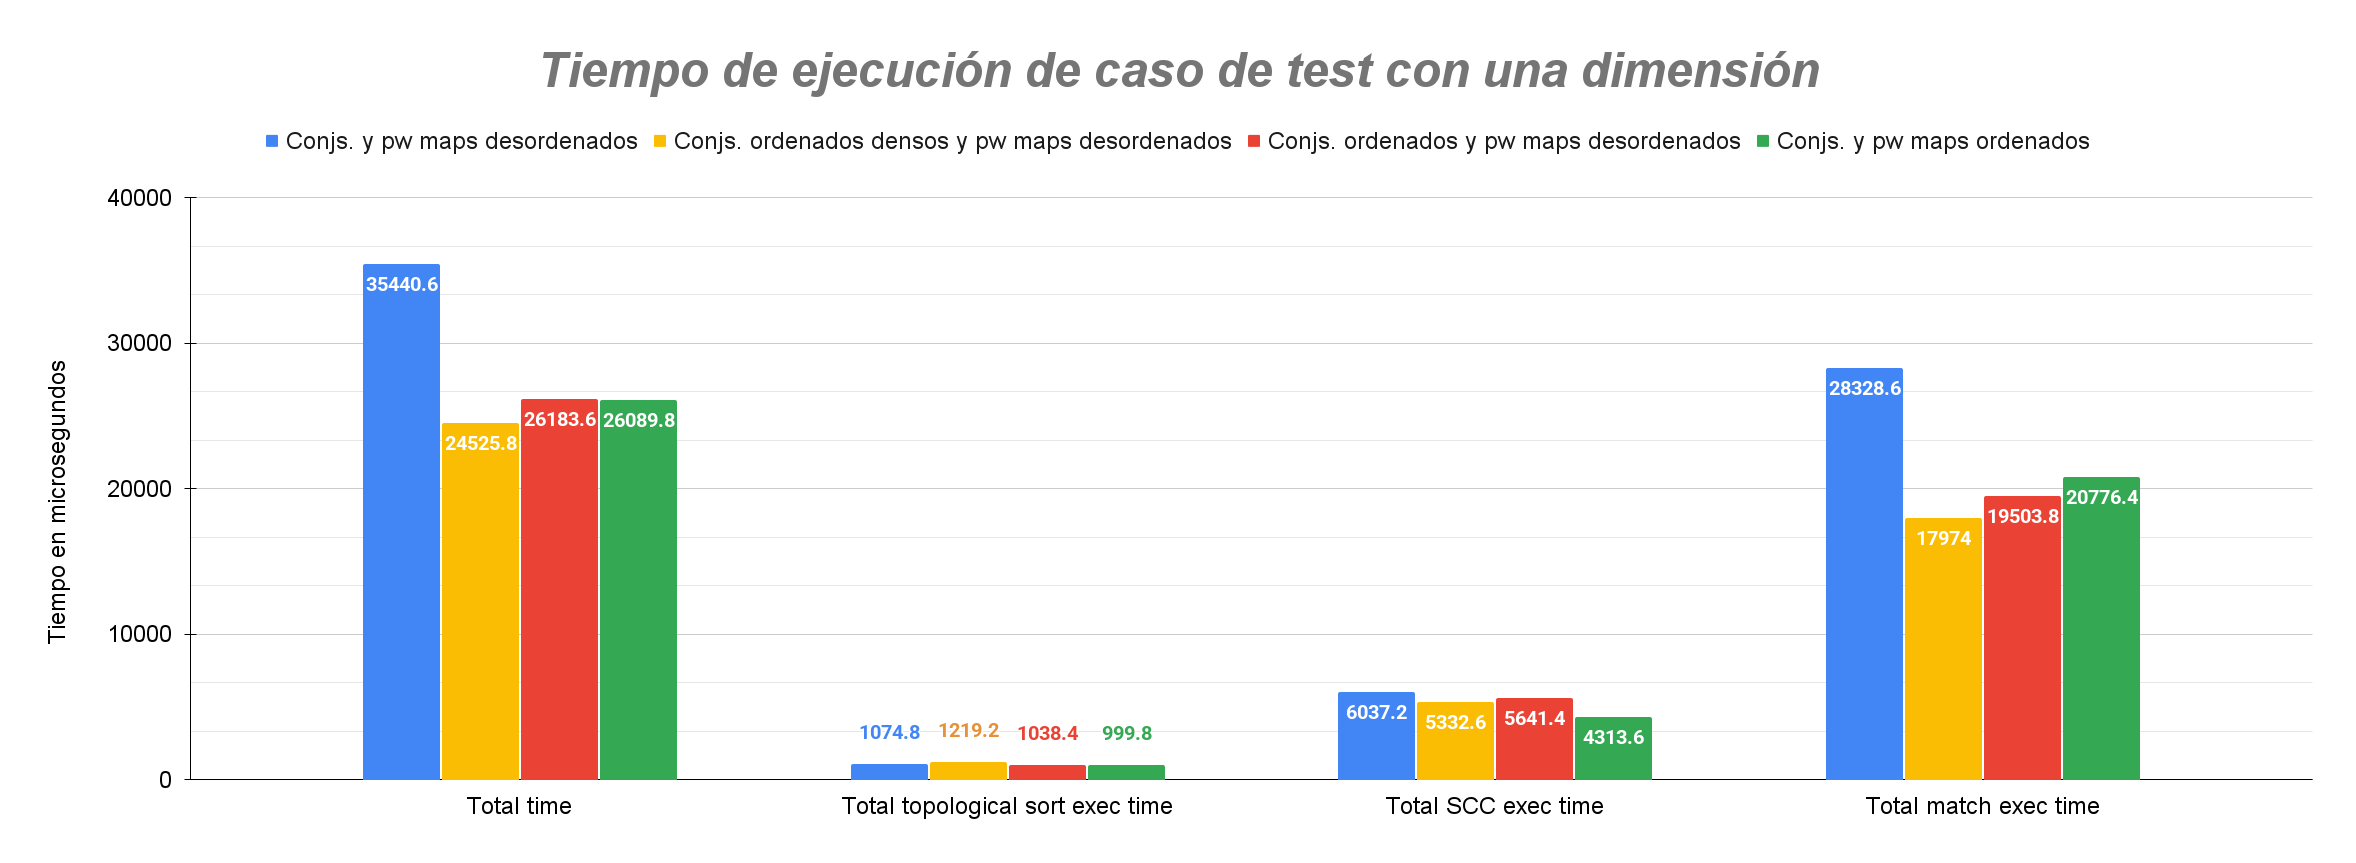
\includegraphics[width=1\linewidth]{figures/Rendimiento/casos de prueba/Tiempo de ejecución de caso de test con una dimensión.png}}
  \caption{Comparación de los diferentes tiempos de ejecución de las diferentes versiones planteadas bajo un caso de prueba en una dimensión.}
  \label{fig:caso-1dim-general}
\end{figure}


Ahora bien, este caso de prueba está basado en un grafo de tamaño relativamente pequeño, por lo que resulta relevante analizar cómo se comportan las distintas versiones a medida que se incrementa el tamaño del grafo, es decir, cómo escalan.
Para evaluar esto, los casos de prueba considerados utilizan una constante de repetición que toma el grafo original y lo replica la cantidad de veces indicada, generando así un único grafo más grande. De esta manera, es posible observar cómo escalan las diferentes combinaciones al aumentar el tamaño del grafo del caso de prueba.

\subsection{Escalado - Caso de prueba en una dimensión}

Con lo anteriormente mencionado, se procede a realizar un análisis de escalabilidad sobre los cuatro tiempos de ejecución presentados para cada una de las versiones propuestas.


\subsubsection{Escalado del \textit{Total Match exec time}}

En el Cuadro~\ref{tab:caso-1dim-match}
y la Figura~\ref{fig:caso-1dim-match2} se observa cómo escala el \textit{Total Match exec time} a medida que se duplica el tamaño del grafo. Se puede notar que los tiempos de ejecución crecen de forma aproximadamente cuadrática en todas las versiones. Sin embargo, aquellas versiones que incorporan ordenamiento escalan de manera significativamente más lenta que la Versión~0.

A pesar de que las versiones con orden escalan de forma similar entre sí, es importante destacar que su \textit{reducción relativa} respecto a la Versión~0 mejora progresivamente a medida que aumenta el tamaño del grafo. En particular incluso, la Versión~3, la más optimizada, escala aún más lentamente que la Versión~1, lo cual se debe al uso más eficiente de los \textit{piecewise maps} ordenados.

Con un único grafo, las reducciones relativas en el \textit{Total Match exec time} con respecto a la Versión~0 son de un \textbf{22{.}67\%} para la Versión~2 y de un \textbf{53{.}33\%} para la Versión~3. Al llegar a 64 copias del grafo original, estas mejoras aumentan a \textbf{58{.}34\%} y \textbf{65{.}42\%}, respectivamente.

En cuanto a la comparación entre la Versión~3 y la Versión~1, esta última siendo la más optimizada para conjuntos en una dimensión, se observa que en el caso de un solo grafo la Versión~3 rinde peor, con un incremento relativo del \textbf{27{.}27\%}. Sin embargo, al llegar a 64 copias del grafo, la tendencia se revierte y la Versión~3 logra una reducción del \textbf{17{,}68\%} respecto a la Versión~1. Esto sugiere que, a medida que el tamaño del grafo continúe creciendo, esta ventaja relativa debería incrementarse aún más todo gracias a la implementación \textit{piecewise maps} ordenados.

\begin{table}[ht]
\centering
\fbox{%
\begin{tabularx}{0.95\textwidth}{|c|>{\centering\arraybackslash}X|>{\centering\arraybackslash}X|>{\centering\arraybackslash}X|>{\centering\arraybackslash}X|}
\hline
\textbf{} & \multicolumn{4}{c|}{\textbf{\textit{Total Match exec time} en milisegundos}} \\
\hline
\textbf{Cantidad de copias} & \textbf{Versión 0} & \textbf{Versión 1} & \textbf{Versión 2} & \textbf{Versión 3} \\
\hline
1   & 30    & 11    & 22    & 14    \\
\hline
2   & 52    & 46    & 43    & 37    \\
\hline
4   & 141   & 90    & 106   & 90    \\
\hline
8   & 459   & 298   & 323   & 233   \\
\hline
16  & 2811  & 1362  & 1490  & 782   \\
\hline
32  & 8142  & 4107  & 5532  & 3056  \\
\hline
64  & 40422 & 16974 & 16838 & 13975 \\
\hline
\end{tabularx}}
\caption{Cuadro comparativo del \textit{Total Match exec time} de las diferentes versiones planteadas bajo un caso de prueba en una dimensión, variando el tamaño del caso de prueba}
\label{tab:caso-1dim-match}
\end{table}


\begin{figure}[htbp]
  \centering
  \fbox{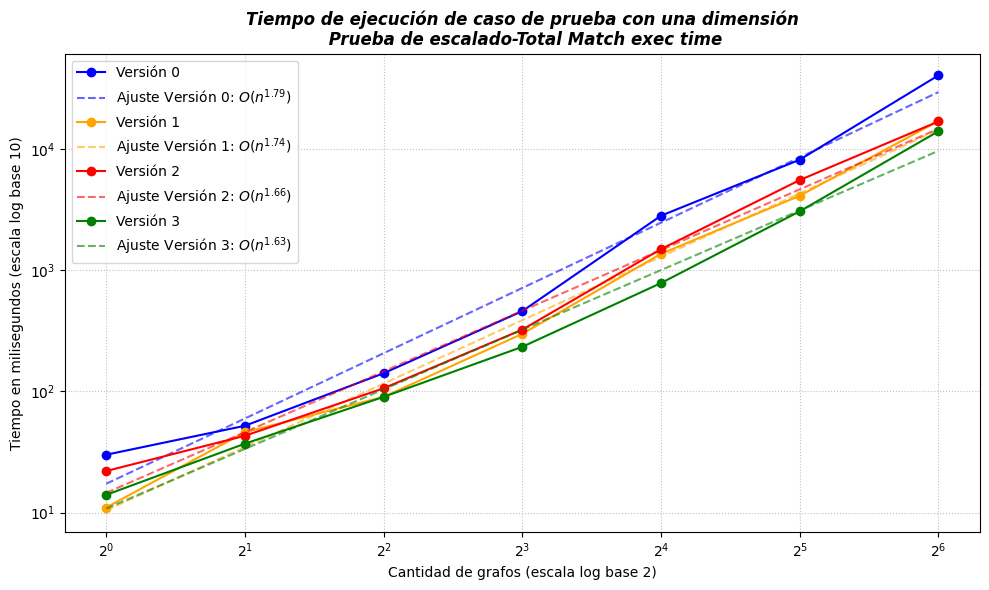
\includegraphics[width=0.9\linewidth]{figures/Rendimiento/casos de prueba/scal3.png}}
  \caption{Gráfico comparativo del \textit{Total Match exec time} de las diferentes versiones planteadas bajo un caso de prueba en una dimensión, variando el tamaño del caso de prueba.}
  \label{fig:caso-1dim-match2}
\end{figure}


\subsubsection{Escalado del \textit{Total SCC exec time}}

En cuanto a este tiempo de ejecución, pueden observarse algunos comportamientos interesantes en el Cuadro~\ref{tab:caso-1dim-scc} y la Figura~\ref{fig:caso-1dim-scc2}. En ella se aprecia nuevamente cómo el tiempo tiende a crecer de forma aproximadamente cuadrática para todas las versiones. Sin embargo, las versiones que incorporan orden muestran un comportamiento particular: aunque resultan más eficientes que la Versión~0, su escalabilidad parece verse afectada por la complejidad del ordenamiento.

Específicamente, a medida que se incrementa el tamaño del grafo, las versiones con mayor manejo de orden escalan de forma menos favorable. En la figura se observa cómo la Versión~2 escala peor que la Versión~1, y a su vez, la Versión~3 escala peor que la Versión~2. Esto puede deberse a como es que utiliza las operaciones disponibles de conjuntos y \textit{piecewise maps} el algoritmo SCC.

Al comienzo, la Versión~2 presenta una reducción relativa del \textbf{57{.}14\%} en comparación con la Versión~1, mientras que la Versión~3 tiene un rendimiento equivalente al de la Versión~2. Sin embargo, al llegar a 64 copias del grafo original, la situación se revierte: la Versión~2 muestra un aumento relativo del \textbf{17{.}45\%} respecto a la Versión~1, y la Versión~3 se comporta aún peor, con un aumento del \textbf{38{.}44\%} en relación con la Versión~2.

\begin{table}[ht]
\centering
\fbox{%
\begin{tabularx}{0.95\textwidth}{|c|>{\centering\arraybackslash}X|>{\centering\arraybackslash}X|>{\centering\arraybackslash}X|>{\centering\arraybackslash}X|}
\hline
\textbf{} & \multicolumn{4}{c|}{\textbf{\textit{Total SCC exec time} en milisegundos}} \\
\hline
\textbf{Cantidad de copias} & \textbf{Versión 0} & \textbf{Versión 1} & \textbf{Versión 2} & \textbf{Versión 3} \\
\hline
1   & 4    & 7    & 3    & 3    \\
\hline
2   & 9    & 5    & 7    & 8    \\
\hline
4   & 19   & 12   & 16   & 19   \\
\hline
8   & 59   & 34   & 46   & 53   \\
\hline
16  & 426  & 233  & 306  & 316  \\
\hline
32  & 975  & 415  & 908  & 781  \\
\hline
64  & 5185 & 1690 & 2046 & 2833 \\
\hline
\end{tabularx}}
\caption{Cuadro comparativo del \textit{Total SCC exec time} de las diferentes versiones planteadas bajo un caso de prueba en una dimensión, variando el tamaño del caso de prueba}
\label{tab:caso-1dim-scc}
\end{table}



\begin{figure}[htbp]
  \centering
  \fbox{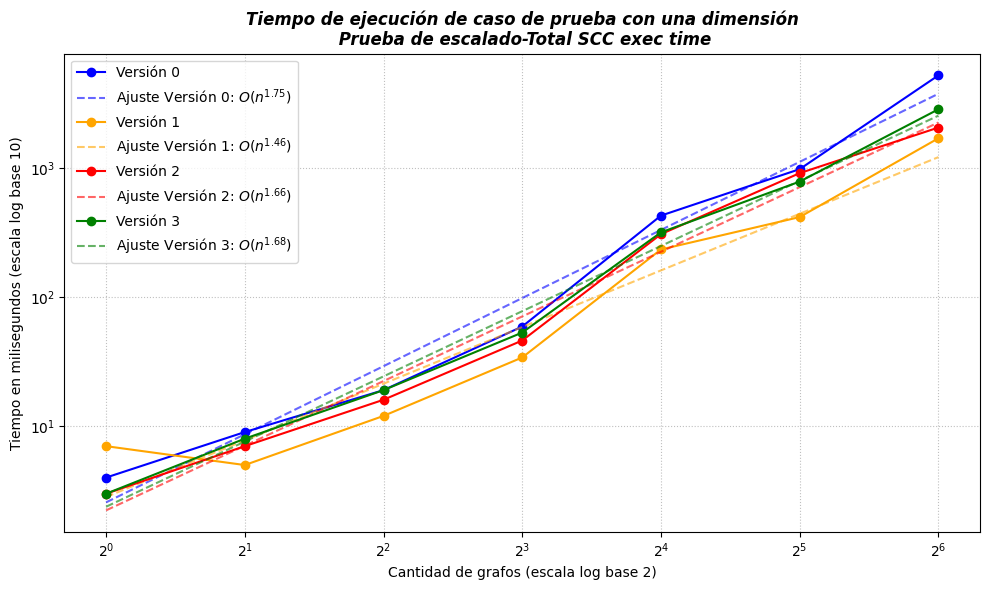
\includegraphics[width=0.9\linewidth]{figures/Rendimiento/casos de prueba/scal4.png}}
  \caption{Gráfico comparativo del \textit{Total SCC exec time} de las diferentes versiones planteadas bajo un caso de prueba en una dimensión, variando el tamaño del caso de prueba.}
  \label{fig:caso-1dim-scc2}
\end{figure}


\subsubsection{Escalado del \textit{Total topological sort exec time}}

En este caso, nuevamente se observan fenómenos relevantes tanto en el Cuadro~\ref{tab:caso-1dim-top} como en la Figura~\ref{fig:caso-1dim-top2}. Los resultados muestran que todas las versiones escalan con una complejidad cercana a la cúbica, lo cual resulta preocupante desde el punto de vista del rendimiento. Este comportamiento indica que, a medida que crece la cantidad de copias del grafo original involucrados, el tiempo de ejecución se incrementa de forma abrupta, lo cual limita la viabilidad de estas implementaciones en contextos de gran escala.

Lo que resulta particularmente llamativo es el hecho de que la Versión~2 presenta un rendimiento aún peor que la Versión~0, lo cual contradice las expectativas, dado que esta última se consideraba como la implementación base o menos optimizada. Solo las Versiones~1 y 3 logran escalar de manera más eficiente que la Versión~0, aunque aun así, sus tasas de crecimiento siguen siendo altas. Esta situación sugiere que, si bien se han logrado algunas mejoras, aún existe un margen considerable para optimizar los algoritmos subyacentes.


\begin{table}[ht]
\centering
\fbox{%
\begin{tabularx}{0.95\textwidth}{|c|>{\centering\arraybackslash}X|>{\centering\arraybackslash}X|>{\centering\arraybackslash}X|>{\centering\arraybackslash}X|}
\hline
\textbf{} & \multicolumn{4}{c|}{\textbf{\textit{Total topological sort exec time} en milisegundos}} \\
\hline
\textbf{Cantidad de copias} & \textbf{Versión 0} & \textbf{Versión 1} & \textbf{Versión 2} & \textbf{Versión 3} \\
\hline
1   & 0     & 1     & 0     & 0     \\
\hline
2   & 3     & 2     & 3     & 4     \\
\hline
4   & 15    & 11    & 15    & 15    \\
\hline
8   & 89    & 85    & 122   & 104   \\
\hline
16  & 682   & 558   & 609   & 974   \\
\hline
32  & 3441  & 3859  & 5107  & 2998  \\
\hline
64  & 25100 & 34945 & 27622 & 22304 \\
\hline
\end{tabularx}}
\caption{Cuadro comparativo del \textit{Total topological sort exec time} de las diferentes versiones planteadas bajo un caso de prueba en una dimensión, variando el tamaño del caso de prueba}
\label{tab:caso-1dim-top}
\end{table}



\begin{figure}[htbp]
  \centering
  \fbox{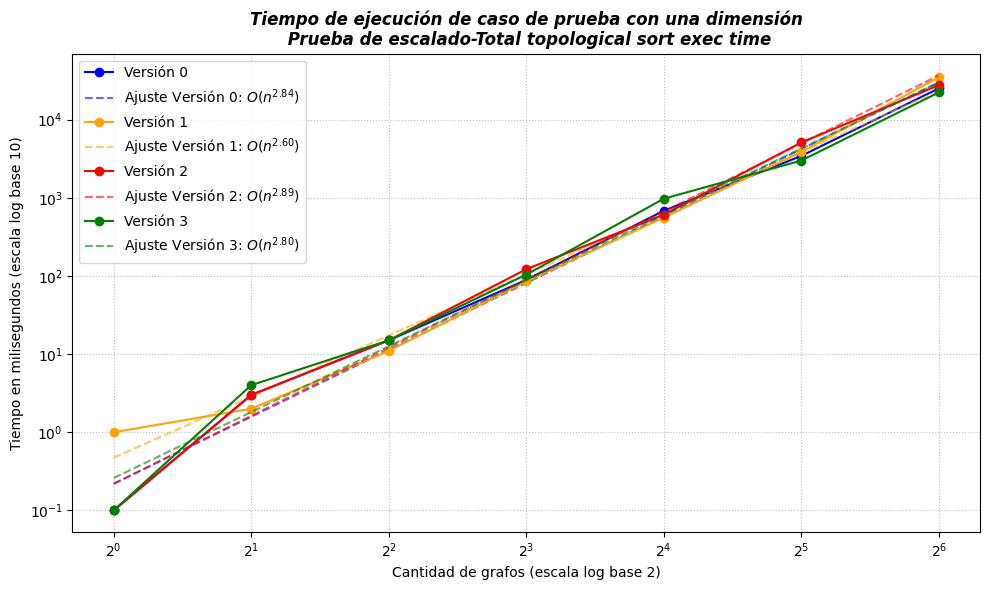
\includegraphics[width=0.9\linewidth]{figures/Rendimiento/casos de prueba/scal5.png}}
  \caption{Gráfico comparativo del \textit{Total topological sort exec time} de las diferentes versiones planteadas bajo un caso de prueba en una dimensión, variando el tamaño del caso de prueba.}
  \label{fig:caso-1dim-top2}
\end{figure}


\subsubsection{Escalado del \textit{Total time}}

Por último, se presenta el tiempo total de ejecución, o \textit{Total time}, el cual se obtiene al sumar todos los tiempos anteriores. De esta manera, es posible analizar cómo escala la ejecución completa del caso de prueba. En el Cuadro~\ref{tab:caso-1dim-total} y la Figura~\ref{fig:caso-1dim-total2} se observan los escalados correspondientes a las distintas versiones propuestas.

En este caso, se aprecia un comportamiento muy particular, con un escalado aproximadamente cuadrático para todas las Versiones, donde las versiones ordenadas superan por muy poco o incluso igualan el escalado de la Versión~0. Adicionalmente, puede notarse que la Versión~3 es la que mejor se desempeña al alcanzar el máximo número de copias del grafo original, obteniendo una reducción relativa del \textbf{44{.}69\%}, \textbf{27{.}03\%} y \textbf{15{.}88\%} en comparación con las Versiones~0, 1 y 2, respectivamente. Claramente cuanto mejor escalen las Versiones mas se acrecentara la reducción relativa, o aumento relativo, entre las mismas a medida que crezca la cantidad de copias, pero como aquí no escalan tan distinto, las reducciones o aumentos no cambian demasiado.

\begin{table}[ht]
\centering
\fbox{%
\begin{tabularx}{0.95\textwidth}{|c|>{\centering\arraybackslash}X|>{\centering\arraybackslash}X|>{\centering\arraybackslash}X|>{\centering\arraybackslash}X|}
\hline
\textbf{} & \multicolumn{4}{c|}{\textbf{\textit{Total time} en milisegundos}} \\
\hline
\textbf{Cantidad de copias} & \textbf{Versión 0} & \textbf{Versión 1} & \textbf{Versión 2} & \textbf{Versión 3} \\
\hline
1   & 34    & 19    & 25    & 17    \\
\hline
2   & 64    & 53    & 53    & 49    \\
\hline
4   & 175   & 113   & 137   & 124   \\
\hline
8   & 607   & 417   & 491   & 390   \\
\hline
16  & 3919  & 2153  & 2405  & 2072  \\
\hline
32  & 12558 & 8381  & 11547 & 6835  \\
\hline
64  & 70707 & 53609 & 46506 & 39112 \\
\hline
\end{tabularx}}
\caption{Cuadro comparativo del \textit{Total time} de las diferentes versiones planteadas bajo un caso de prueba en una dimensión, variando el tamaño del caso de prueba}
\label{tab:caso-1dim-total}
\end{table}



\begin{figure}[htbp]
  \centering
  \fbox{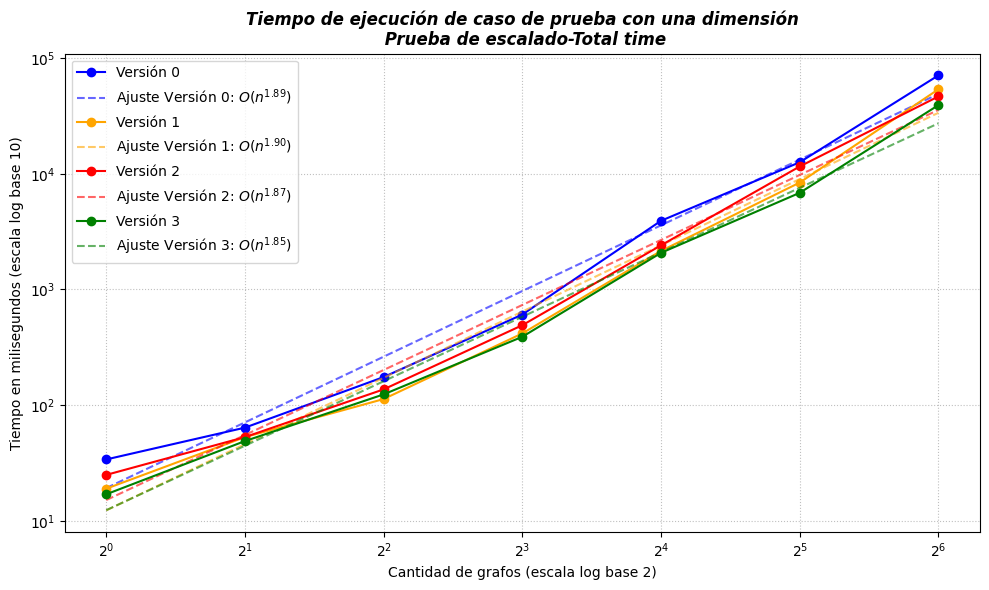
\includegraphics[width=0.9\linewidth]{figures/Rendimiento/casos de prueba/scal6.png}}
  \caption{Gráfico comparativo del \textit{Total time} de las diferentes versiones planteadas bajo un caso de prueba en una dimensión, variando el tamaño del caso de prueba.}
  \label{fig:caso-1dim-total2}
\end{figure}


\subsection{Caso de prueba en dos dimensiones}

Ahora bien, al trabajar únicamente con una sola dimensión, no se está aprovechando completamente las optimizaciones implementadas tanto en los conjuntos como en los \textit{piecewise maps} ordenados. Es por ello que a continuación se presentará un nuevo caso de prueba, esta vez en dos dimensiones. El código correspondiente se encuentra disponible en el archivo \textit{pw\_map\_test\_2dim.test}, ubicado en la carpeta \textit{test} dentro del repositorio.

Cabe destacar que, en esta ocasión, no se dispone del valor correspondiente a \textit{Total topological sort exec time}, por lo que dicho tiempo de ejecución será omitido tanto en el análisis como en el cálculo del \textit{Total time}.

En la Figura~\ref{fig:caso-2dim-general} se presentan los diferentes tiempos de ejecución analizados en este caso para todas las versiones, con excepción de la Versión~1, la cual solo es válida en el contexto unidimensional. Nuevamente los valores resultan el promedio de múltiples ejecuciones para cada una de las versiones. A partir de este gráfico, pueden destacarse las siguientes observaciones:

\begin{itemize}
    \item Las versiones que incorporan orden en su implementación resultan más eficientes que la Versión~0, especialmente en lo que respecta al \textit{Total match exec time}. En particular, se observa una reducción relativa del \textbf{30{.}70\%} y \textbf{43{.}74\%} para las Versiones~2 y~3, respectivamente.

    \item De forma similar, se evidencia una disminución en el \textit{Total SCC exec time}, con reducciones relativas del \textbf{29{.}96\%} y \textbf{38{.}87\%} para las Versiones~2 y~3 en comparación con la Versión~0.

    \item En cuanto al \textit{Total time}, se registra una mejora general con reducciones relativas del \textbf{30{.}61\%} y \textbf{42{.}87\%} también para las Versiones~2 y~3 respecto a la Versión~0.
\end{itemize}


\begin{figure}[htbp]
  \centering
  \fbox{\includegraphics[width=1\linewidth]{figures/Rendimiento/casos de prueba/Tiempo de ejecución de caso de test con dos dimensiones.png}}
  \caption{Comparación de los tiempos de ejecución de las diferentes versiones planteadas bajo un caso de prueba en dos dimensiones.}
  \label{fig:caso-2dim-general}
\end{figure}

\subsection{Escalado - Caso de prueba en dos dimensiones}

Nuevamente se chequeará cómo es que escalan los tiempos de ejecución a medida de que el grafo crece en tamaño. A continuación, se analizará cada una de las medidas por separado.

\subsubsection{Escalado del \textit{Total Match exec time}}

Como se observa en el Cuadro~\ref{tab:caso-2dim-match} y en la Figura~\ref{fig:caso-2dim-match2}, en esta ocasión el tiempo de ejecución presenta un comportamiento que escala de forma cuadrática o incluso peor en el caso de la Versión~0. En cambio, las Versiones~2 y~3 muestran un crecimiento subcuadrático, destacándose la Versión~3 como la más eficiente.

En particular, para el caso más simple con una sola copia del grafo original, se observa una reducción relativa del \textbf{31{.}86\%} y \textbf{34{.}51\%} en las Versiones~2 y~3, respectivamente, en comparación con la Versión~0. Esta mejora se vuelve aún más significativa a medida que crece el grafo, ya que con 32 copias, la reducción alcanza el \textbf{76{.}54\%} para la Versión~2 y el \textbf{81{.}86\%} para la Versión~3, siendo \textbf{4{.}26} veces y \textbf{5{.}51} veces mas rápidas respectivamente que la Versión~0.

\begin{table}[ht]
\centering
\fbox{%
\begin{tabularx}{0.9\textwidth}{|c|>{\centering\arraybackslash}X|>{\centering\arraybackslash}X|>{\centering\arraybackslash}X|}
\hline
\textbf{} & \multicolumn{3}{c|}{\textbf{\textit{Total Match exec time} en milisegundos}} \\
\hline
\textbf{Cantidad de copias} & \textbf{Versión 0} & \textbf{Versión 2} & \textbf{Versión 3} \\
\hline
1   & 113    & 77     & 74     \\
\hline
2   & 389    & 241    & 200    \\
\hline
4   & 1549   & 802    & 663    \\
\hline
8   & 7842   & 2951   & 2127   \\
\hline
16  & 31561  & 11212  & 9066   \\
\hline
32  & 184108 & 43177  & 33401  \\
\hline
\end{tabularx}}
\caption{Cuadro comparativo del \textit{Total Match exec time} de las diferentes versiones planteadas bajo un caso de prueba en dos dimensiones, variando el tamaño del caso de prueba}
\label{tab:caso-2dim-match}
\end{table}



\begin{figure}[htbp]
  \centering
  \fbox{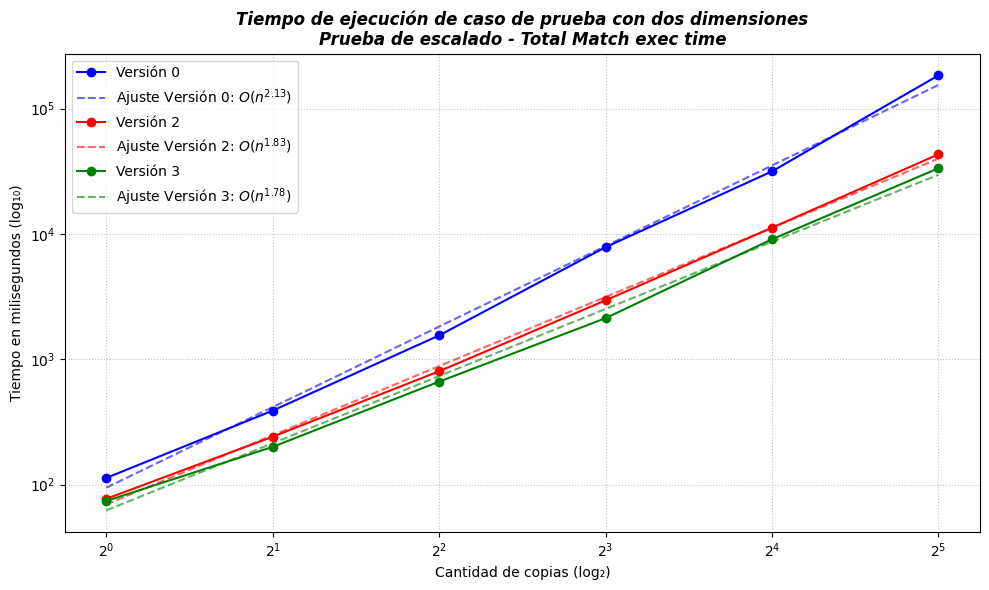
\includegraphics[width=0.9\linewidth]{figures/Rendimiento/casos de prueba/scal7.png}}
  \caption{Gráfico comparativo del \textit{Total Match exec time} de las diferentes versiones planteadas bajo un caso de prueba en dos dimensiones, variando el tamaño del caso de prueba.}
  \label{fig:caso-2dim-match2}
\end{figure}



\subsubsection{Escalado del \textit{Total SCC exec time}}

En esta ocasión, en la Figura~\ref{fig:caso-2dim-scc2} y en el Cuadro~\ref{tab:caso-2dim-scc}, se observa una situación particular. Aunque nuevamente el escalado general parece similar al visto en el \textit{Total Match exec time}, en este caso no es la Versión~3 la que presenta el mejor escalabilidad, sino la Versión~2.

Esta diferencia podría explicarse por el tipo de operaciones utilizadas en la implementación con \textit{piecewise maps} ordenados, las cuales podrían estar introduciendo una sobrecarga adicional que afecta el tiempo de ejecución, a pesar de las mejoras estructurales de dicha versión.

\begin{table}[ht]
\centering
\fbox{%
\begin{tabularx}{0.9\textwidth}{|c|>{\centering\arraybackslash}X|>{\centering\arraybackslash}X|>{\centering\arraybackslash}X|}
\hline
\textbf{} & \multicolumn{3}{c|}{\textbf{\textit{Total SCC exec time} en milisegundos}} \\
\hline
\textbf{Cantidad de copias} & \textbf{Versión 0} & \textbf{Versión 2} & \textbf{Versión 3} \\
\hline
1   & 25    & 17    & 19    \\
\hline
2   & 64    & 45    & 51    \\
\hline
4   & 477   & 144   & 302   \\
\hline
8   & 1413  & 429   & 477   \\
\hline
16  & 3597  & 896   & 1462  \\
\hline
32  & 20215 & 3435  & 3939  \\
\hline
\end{tabularx}}
\caption{Cuadro comparativo del \textit{Total SCC exec time} de las diferentes versiones planteadas bajo un caso de prueba en dos dimensiones, variando el tamaño del caso de prueba}
\label{tab:caso-2dim-scc}
\end{table}


    
\begin{figure}[htbp]
  \centering
  \fbox{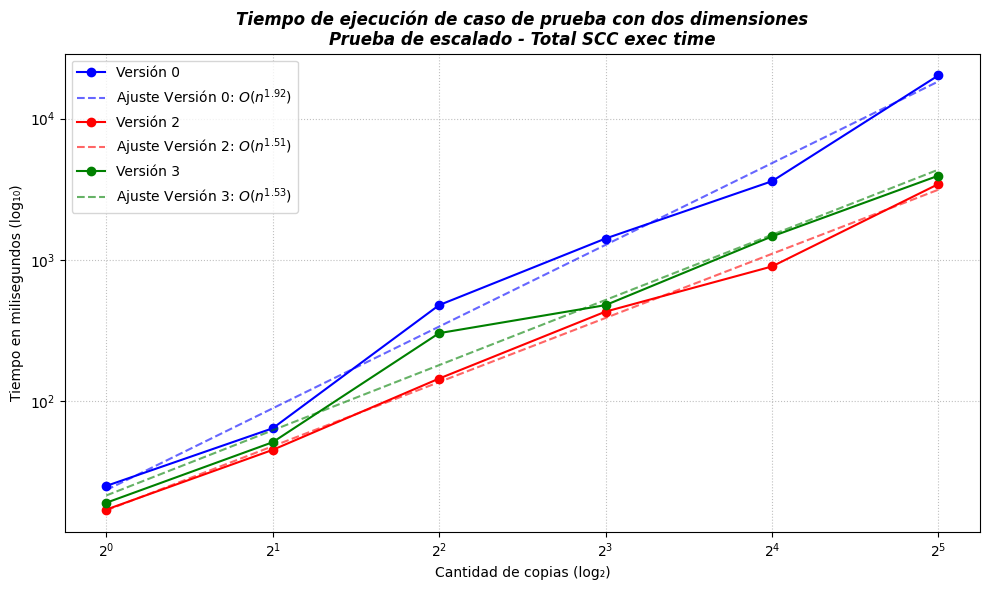
\includegraphics[width=0.9\linewidth]{figures/Rendimiento/casos de prueba/scal8.png}}
  \caption{Gráfico comparativo del \textit{Total SCC exec time} de las diferentes versiones planteadas bajo un caso de prueba en dos dimensiones, variando el tamaño del caso de prueba.}
  \label{fig:caso-2dim-scc2}
\end{figure}



\subsubsection{Escalado del \textit{Total time}}

Como era de esperarse en base a los resultados anteriores, en el Cuadro~\ref{tab:caso-2dim-total} y en la Figura~\ref{fig:caso-2dim-total2} se puede evidenciar que se repite el mismo patrón observado en el análisis de escalado del \textit{Total Match exec time}. En esta oportunidad, la diferencia relativa respecto a la Versión~0 alcanza un \textbf{77{.}19\%} en el caso de la Versión~2 y un \textbf{81{.}73\%} para la Versión~3 con el máximo de cantidad de copias del grafo original, confirmando nuevamente la eficacia de las optimizaciones implementadas. En este caso, dado que la diferencia de escalado con respecto a la Versión~0 es considerablemente mayor, al aumentar la cantidad de copias estas diferencias tenderían a incrementarse aún más. Lo mismo ocurre al comparar la Versión~2 con la Versión~3, donde también se espera que la reducción relativa se amplíe.


\begin{table}[ht]
\centering
\fbox{%
\begin{tabularx}{0.9\textwidth}{|c|>{\centering\arraybackslash}X|>{\centering\arraybackslash}X|>{\centering\arraybackslash}X|}
\hline
\textbf{} & \multicolumn{3}{c|}{\textbf{\textit{Total time} en milisegundos}} \\
\hline
\textbf{Cantidad de copias} & \textbf{Versión 0} & \textbf{Versión 2} & \textbf{Versión 3} \\
\hline
1   & 138    & 94     & 93     \\
\hline
2   & 453    & 286    & 251    \\
\hline
4   & 2026   & 946    & 965    \\
\hline
8   & 9255   & 3380   & 2604   \\
\hline
16  & 35158  & 12108  & 10528  \\
\hline
32  & 204323 & 46612  & 37340  \\
\hline
\end{tabularx}}
\caption{Cuadro comparativo del \textit{Total time} de las diferentes versiones planteadas bajo un caso de prueba en dos dimensiones, variando el tamaño del caso de prueba}
\label{tab:caso-2dim-total}
\end{table}


\begin{figure}[htbp]
  \centering
  \fbox{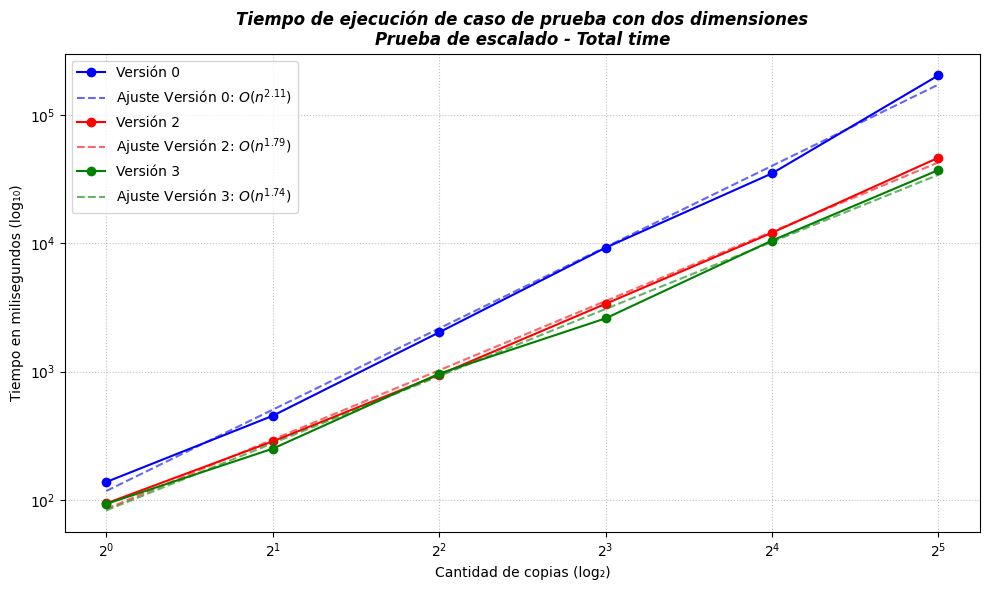
\includegraphics[width=0.9\linewidth]{figures/Rendimiento/casos de prueba/scal9.png}}
  \caption{Gráfico comparativo del \textit{Total time} de las diferentes versiones planteadas bajo un caso de prueba en dos dimensiones, variando el tamaño del caso de prueba.}
  \label{fig:caso-2dim-total2}
\end{figure}

